\documentclass[11pt,a4paper]{article}

\usepackage[margin=1in]{geometry}
\usepackage[T1]{fontenc}
\usepackage{lmodern}
\usepackage{amsmath,amssymb}
\usepackage{graphicx}
\usepackage{tikz}
\usepackage{booktabs}
\usepackage{hyperref}
\usepackage{parskip}
\usepackage{enumitem}
\usepackage{xcolor}
\definecolor{gold}{rgb}{0.85,0.65,0.13}

\hypersetup{colorlinks=true, linkcolor=blue!60!black, urlcolor=blue!60!black}

\title{\textbf{Research Companion Guide}\\[6pt]
\large A Comprehensive Explanation of\\[3pt]
\emph{A Morphological Barrier: Quantifying the Injection Realism Gap\\for CNN Strong Lens Finders in DESI Legacy Survey DR10}}
\author{Companion to the research paper (v16)}
\date{February 2026}

\begin{document}
\maketitle
\thispagestyle{empty}

\vspace{1cm}
\noindent\textbf{What this document is.}
This is a self-contained guide that explains every aspect of the research paper in accessible language.
It covers the astrophysics background, the statistical methods, the experimental design, the results,
and how to defend the work in conversation.
Every technical term is defined when first used.
Numbers are cited exactly as they appear in the paper.
Analogies are used but clearly marked.
Limitations are stated honestly.

\noindent\textbf{How to use it.}
Part~I provides background you need before reading the paper.
Part~II walks through what we did, section by section.
Part~III explains what it means and how to defend it.
Each chapter begins with a brief summary of what you will learn.

\newpage
\tableofcontents
\newpage

% ====================================================================
% PART I
% ====================================================================
\part{Background You Need}

\section{Chapter 1: Gravitational Lensing from Scratch}

\textit{In this chapter you will learn what gravitational lensing is, why massive galaxies bend light, what the Einstein radius means, and what real strong lenses look like on the sky.}

\subsection{What Gravity Does to Light}

Einstein's theory of general relativity predicts that massive objects curve spacetime. Light rays follow these curved paths, so a massive object between you and a distant source can bend the light and change how and where you see it. In other words, gravity bends light.

This idea was first confirmed during the 1919 solar eclipse. Arthur Eddington measured the apparent positions of stars near the Sun's limb and found their positions shifted by about the amount Einstein predicted. Light from those stars was bent as it passed the Sun on its way to Earth. Gravity really does curve light.

You can picture this like a bowling ball on a trampoline. Rolling a marble past the ball makes its path curve toward the center. Light behaves similarly: its path curves as it passes near massive objects such as stars and galaxies.

\subsection{Strong, Weak, and Micro Lensing}

Not all lensing looks the same. Three regimes matter:

\textbf{Strong lensing} is the regime where the bending is large enough to produce multiple, well-separated images or arcs. Imagine looking at a distant streetlight through the stem of a wine glass: the light can split into several distinct images. Strong lensing works the same way: one background galaxy can appear as two, three, or four separate images, or as arcs and rings.

\textbf{Weak lensing} produces only small distortions---typically a few percent---so you usually cannot see multiple images. Instead, shapes are slightly stretched or sheared. Think of looking through slightly warped glass: things look nearly normal but subtly distorted. Weak lensing is used to measure mass distributions in galaxy clusters and for cosmology.

\textbf{Micro lensing} occurs when the lens is so small (e.g., a star or planet) that you do not resolve separate images. You only see a temporary brightening as the lens moves across the line of sight. It is like a magnifying glass briefly passing in front of a light: you notice the change in brightness rather than multiple images.

This guide focuses on \emph{strong} lensing, where the lens is typically a massive galaxy.

\subsection{The Einstein Radius}

The \textbf{Einstein radius} is a key concept. Imagine a distant galaxy exactly behind a foreground galaxy, along your line of sight. In that perfectly aligned case, the background galaxy would appear as a ring around the lens. The angular radius of that ring (measured on the sky in arcseconds) is the Einstein radius, usually denoted $\theta_E$.

Physically, the Einstein radius marks the scale over which gravity is strong enough to produce multiple images or arcs. If the source sits inside this radius (in angular terms), you tend to get arcs or rings; if it sits outside, you get multiple images.

For galaxy-scale lenses, typical Einstein radii are in the range 0.5--3~arcseconds. One arcsecond is about $1/3600$ of a degree. That is tiny on the sky, but modern telescopes and cameras can resolve it.

\subsection{What Real Strong Lenses Look Like}

Real strong lenses do not always show perfect rings. What you see depends on alignment:

\textbf{Einstein rings} occur when the source is almost perfectly aligned with the lens. You see a smooth or nearly complete ring of light around the lens galaxy.

\textbf{Arcs} (partial rings) appear when the source is slightly offset. Part of the ring is brighter or more extended than the rest, so you see arc-shaped structures.

\textbf{Multiple images} appear when the source is farther from perfect alignment. Instead of a ring or arcs, you see two, three, or four distinct images of the same background galaxy around the lens.

The lens galaxy itself usually appears as a bright blob in the center. The lensed images and arcs sit around it, often reddish or bluish depending on the colors of the lens and source galaxies.

\subsection{Why Massive Elliptical Galaxies Are the Best Lenses}

Strong lensing is dominated by \textbf{elliptical galaxies}---roundish, reddish systems without spiral arms. The main reason is mass. The lensing ``strength'' scales with mass. The more mass between you and the source, the more bending and the larger the Einstein radius. Elliptical galaxies are typically the most massive galaxies in the universe, so they bend light the most.

\subsection{Source Plane and Image Plane}

Two planes help organize the geometry:

The \textbf{source plane} is the plane in 3D space where the background galaxy actually lies. Think of it as the ``true'' location of the source.

The \textbf{image plane} is the plane of the sky where we observe the light---the 2D view from Earth. The lens bends light from the source plane to create the pattern we see in the image plane.

\begin{center}
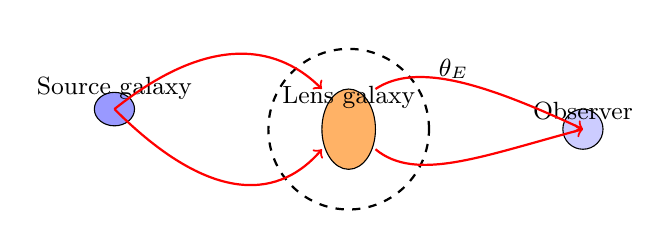
\begin{tikzpicture}[scale=0.85, every node/.style={font=\small}]
  \coordinate (observer) at (7, 0);
  \coordinate (lens) at (3.5, 0);
  \coordinate (source) at (0, 0.3);
  \draw[fill=blue!20] (observer) circle (0.3);
  \node[above] at (observer) {Observer};
  \draw[fill=orange!60] (lens) ellipse (0.4 and 0.6);
  \node[above=4pt] at (lens) {Lens galaxy};
  \draw[dashed, thick] (lens) circle (1.2);
  \node[right] at (4.7, 0.9) {$\theta_E$};
  \draw[fill=blue!40] (source) ellipse (0.3 and 0.25);
  \node[above] at (source) {Source galaxy};
  \draw[->, thick, red] (source) .. controls (1.5, 1.5) and (2.5, 1.2) .. (3.1, 0.6);
  \draw[->, thick, red] (3.9, 0.6) .. controls (4.5, 1.0) and (5.5, 0.7) .. (observer);
  \draw[->, thick, red] (source) .. controls (1.5, -1.2) and (2.5, -1.0) .. (3.1, -0.3);
  \draw[->, thick, red] (3.9, -0.3) .. controls (4.5, -0.8) and (5.5, -0.4) .. (observer);
\end{tikzpicture}
\end{center}

The diagram shows the basic setup: observer on the right, lens in the middle, source on the left. The dashed circle marks the Einstein radius $\theta_E$. Red curves show light rays bending around the lens on their way to the observer.


\section{Chapter 2: Why Astronomers Care About Finding Lenses}

\textit{In this chapter you will learn why strong lenses matter for cosmology and dark matter, what a selection function is, how injection-recovery works, and why the central question of our paper---whether fake lenses look realistic---matters for all of this.}

\subsection{Population Statistics}

Finding strong lenses is useful not only individually, but also as a population. If you know how many lenses exist with certain properties (Einstein radius, redshift, mass, etc.), you can test models of galaxy formation, dark matter, and cosmology. Comparing observed lens counts to theoretical predictions constrains the mass function of galaxies and the geometry of the universe.

\subsection{Connection to Dark Matter, Cosmology, and Galaxy Evolution}

Strong lensing depends on total mass---stars, gas, and dark matter. That makes it a direct probe of dark matter distribution.

\textbf{Time delays} add another dimension. Light traveling along different paths can take different times to reach us. Measuring these delays and modeling the lens gives a physical distance, which can be combined with redshift to estimate the Hubble constant $H_0$---the expansion rate of the universe.

Lensed systems also magnify distant galaxies, revealing fainter objects and earlier stages of galaxy evolution.

\subsection{The Selection Function Concept}

If you find 100 lenses, how many did you miss? That question is critical for population statistics.

The \textbf{selection function} is the probability that a lens with given properties is detected by your survey and pipeline. It depends on flux, size, morphology, image quality, and the algorithm used. Without it, you cannot correct for incompleteness or turn ``lenses found'' into ``lenses present.''

\subsection{The Injection-Recovery Paradigm}

A standard way to estimate the selection function is \textbf{injection-recovery}:
\begin{enumerate}
  \item Create synthetic (simulated) lenses with known properties.
  \item Insert them into real survey images at random positions.
  \item Run your detection pipeline (e.g., a CNN) on these images.
  \item Measure what fraction you recover, as a function of those properties.
\end{enumerate}
That recovery fraction is your empirical selection function.

\subsection{The Critical Assumption}

Injection-recovery works \emph{only} if the synthetic lenses are representative of real ones. If synthetic and real lenses differ in ways that affect detectability, the measured selection function will be wrong, and so will any population inferences.

\textbf{This is the central question of our paper}: Do synthetic lenses used in injection-recovery look sufficiently like real lenses to the CNN? If not, the selection function and the population statistics built on it may be biased.


\section{Chapter 3: How CNNs See Images}

\textit{In this chapter you will learn what a convolutional neural network is, how it processes images through layers of filters, what embeddings and feature space mean, and how the CNN outputs a detection score.}

\subsection{Neural Networks}

\textbf{Neural networks} are algorithms inspired by networks of neurons in the brain. They consist of layers of simple mathematical operations: each ``neuron'' takes inputs, applies weights and a nonlinear function, and passes the result to the next layer. With enough layers and proper training, such networks can learn to approximate complex input--output relationships.

\subsection{Convolutional Neural Networks}

\textbf{Convolutional neural networks} (CNNs) are built for images. They use small \textbf{filters} (or \textbf{kernels})---arrays of numbers, e.g., $3 \times 3$ or $5 \times 5$---that slide across the image. Each filter responds to certain local patterns (edges, corners, textures). Many filters in many layers allow the network to build up increasingly complex descriptions of the image.

\subsection{Hierarchy of Features}

CNNs typically learn a hierarchy:
\begin{itemize}
  \item \textbf{Early layers}: edges, gradients, simple shapes.
  \item \textbf{Middle layers}: textures, combinations of edges, more complex shapes.
  \item \textbf{Deep layers}: high-level concepts such as ``galaxy,'' ``arc,'' or ``ring.''
\end{itemize}

\subsection{EfficientNetV2-S}

\textbf{EfficientNetV2-S} is our CNN architecture with about 20.2 million parameters. It was \textbf{pre-trained} on \textbf{ImageNet}---a large dataset of everyday photos---then \textbf{fine-tuned} on astronomical images.

\subsection{Transfer Learning}

\textbf{Transfer learning} means starting from a model trained on one domain and adapting it to another. Low-level visual features---edges, textures, contrast---are shared across domains. A network trained on natural images already has useful edge and texture detectors; fine-tuning adjusts them for astronomical data.

\subsection{Embeddings and Feature Space}

Before the final classification, the CNN produces an \textbf{embedding}---a vector of 1280 numbers that summarizes what the network ``sees'' in the image. This is the \textbf{feature space}: each image is a point in 1280-dimensional space. Images that look similar to the CNN have similar embeddings.

\subsection{Binary Classification}

The final layer maps the 1280-d embedding to a single number $p$ between 0 and 1: the probability the image is a lens. $p \approx 1$ means ``likely a lens''; $p \approx 0$ means ``likely not.''

\begin{center}
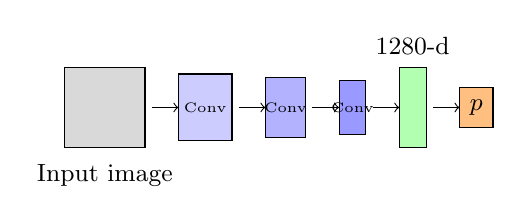
\begin{tikzpicture}[scale=0.85, every node/.style={font=\small}]
  \draw[fill=gray!30] (0, 0) rectangle (1.2, 1.2);
  \node[below] at (0.6, -0.1) {Input image};
  \draw[->] (1.3, 0.6) -- (1.7, 0.6);
  \draw[fill=blue!20] (1.7, 0.1) rectangle (2.5, 1.1);
  \node at (2.1, 0.6) {\tiny Conv};
  \draw[->] (2.6, 0.6) -- (3.0, 0.6);
  \draw[fill=blue!30] (3.0, 0.15) rectangle (3.6, 1.05);
  \node at (3.3, 0.6) {\tiny Conv};
  \draw[->] (3.7, 0.6) -- (4.1, 0.6);
  \draw[fill=blue!40] (4.1, 0.2) rectangle (4.5, 1.0);
  \node at (4.3, 0.6) {\tiny Conv};
  \draw[->] (4.6, 0.6) -- (5.0, 0.6);
  \draw[fill=green!30] (5.0, 0.0) rectangle (5.4, 1.2);
  \node[above] at (5.2, 1.25) {1280-d};
  \draw[->] (5.5, 0.6) -- (5.9, 0.6);
  \draw[fill=orange!50] (5.9, 0.3) rectangle (6.4, 0.9);
  \node at (6.15, 0.6) {$p$};
\end{tikzpicture}
\end{center}

\begin{center}
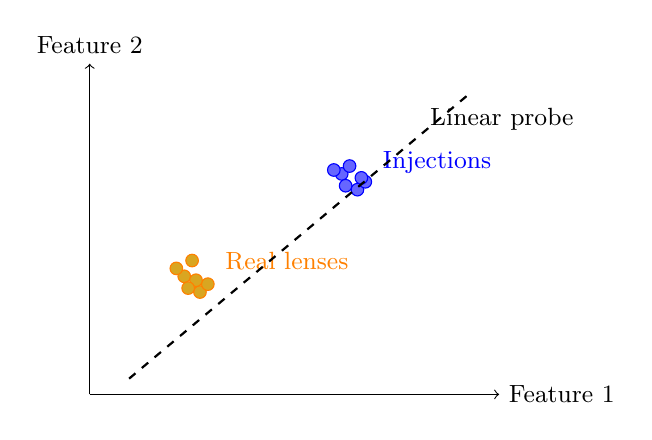
\begin{tikzpicture}[scale=1, every node/.style={font=\small}]
  \draw[->] (0, 0) -- (5.2, 0) node[right] {Feature 1};
  \draw[->] (0, 0) -- (0, 4.2) node[above] {Feature 2};
  \foreach \x/\y in {1.2/1.5, 1.4/1.3, 1.3/1.7, 1.5/1.4, 1.1/1.6, 1.35/1.45, 1.25/1.35}
    {\draw[fill=gold, draw=orange] (\x, \y) circle (0.08);}
  \node[right] at (1.6, 1.7) {\color{orange} Real lenses};
  \foreach \x/\y in {3.2/2.8, 3.4/2.6, 3.3/2.9, 3.5/2.7, 3.1/2.85, 3.45/2.75, 3.25/2.65}
    {\draw[fill=blue!60, draw=blue] (\x, \y) circle (0.08);}
  \node[right] at (3.6, 2.95) {\color{blue} Injections};
  \draw[dashed, thick] (0.5, 0.2) -- (4.8, 3.8);
  \node[right] at (4.2, 3.5) {Linear probe};
\end{tikzpicture}
\end{center}

The feature-space diagram shows a 2D analogy. Gold dots are real lenses; blue dots are injections. They cluster in different regions. The dashed line is the \textbf{linear probe}---a simple boundary that separates them. If a simple straight line can do this, the CNN has learned features that make real and synthetic lenses fundamentally different.


% ====================================================================
% CHAPTERS 4-6 (statistics, DESI, prior work)
% ====================================================================
% LaTeX body content for Part I, Chapters 4-6
% Research Companion Guide - CNN Strong Gravitational Lens Finding
% No preamble, no \part, no \begin{document} - start with \section

\section{Chapter 4: Statistics Toolkit}

This chapter explains the statistical tools we use to evaluate our CNN lens finder and to diagnose whether our simulated lens injections look realistic. We build each concept from first principles and include worked examples so you can follow the logic step by step.

\subsection{The ROC Curve and AUC}

\subsubsection{What Is a Classifier Threshold?}

When a CNN looks at an image, it outputs a \textbf{score}---a number between 0 and 1---that represents how confident it is that the image shows a strong lens. But a score alone does not make a decision. We need a \textbf{threshold}: a cutoff value $p^*$ such that we call everything with score $\geq p^*$ a ``positive'' (lens) and everything below a ``negative'' (non-lens).

For example, if $p^* = 0.5$, then any image with score $\geq 0.5$ is classified as a lens. If $p^* = 0.9$, we are stricter: only very high scores count as lenses. Changing the threshold changes how many lenses we find and how many false alarms we accept. There is a trade-off: lower thresholds find more real lenses but also more false positives; higher thresholds miss more lenses but reduce false alarms.

\subsubsection{True Positive Rate and False Positive Rate}

At each threshold $p^*$, we can compute two key rates:

\begin{itemize}
    \item \textbf{True Positive Rate (TPR)}, also called \textbf{recall}: Of all the actual lenses in our data, what fraction did we correctly classify as lenses? If we have 100 real lenses and we correctly flag 80 of them, TPR $= 80/100 = 0.80$. Higher TPR means we are finding more of the real lenses.
    \item \textbf{False Positive Rate (FPR)}: Of all the actual non-lenses, what fraction did we wrongly classify as lenses? If we have 1000 non-lenses and 50 of them got high scores and were falsely flagged, FPR $= 50/1000 = 0.05$. Lower FPR means fewer false alarms.
\end{itemize}

As we sweep $p^*$ from 0 to 1, TPR and FPR change. At $p^* = 0$, we call everything a lens, so TPR $= 1$ and FPR $= 1$. At $p^* = 1$, we call almost nothing a lens, so TPR $\approx 0$ and FPR $\approx 0$. In between, we trace out a curve.

\subsubsection{The ROC Curve}

The \textbf{ROC curve} (Receiver Operating Characteristic curve) is a plot of TPR on the vertical axis versus FPR on the horizontal axis, as we sweep the threshold from 0 to 1. Each point on the curve corresponds to one choice of threshold.

A perfect classifier would have TPR $= 1$ and FPR $= 0$ at some threshold: it finds all lenses and zero false alarms. That would trace a curve that goes straight up the left side and then across the top. A useless classifier that randomly guesses would give points along the diagonal line from $(0,0)$ to $(1,1)$: increasing the threshold trades TPR and FPR one-for-one, like flipping a coin.

\subsubsection{AUC: Area Under the Curve}

The \textbf{AUC} (Area Under the ROC Curve) is the area under the ROC curve. It is a single number that summarizes the classifier's performance across all thresholds.

\begin{itemize}
    \item \textbf{AUC $= 1.0$}: Perfect separation. The curve hugs the top-left corner; there exists a threshold where we get all lenses and no false alarms.
    \item \textbf{AUC $= 0.5$}: Random guessing. The curve lies on the diagonal; the classifier adds no information beyond chance.
    \item \textbf{AUC between 0.5 and 1.0}: Some discrimination. The higher the AUC, the better the classifier at ranking lenses above non-lenses.
\end{itemize}

\subsubsection{Intuitive Interpretation of AUC}

A beautiful interpretation: \textbf{AUC is the probability that a randomly chosen positive (lens) gets a higher score than a randomly chosen negative (non-lens)}. If we pick one lens and one non-lens at random and compare their scores, AUC tells us how often the lens wins. AUC $= 0.5$ means they tie on average (random); AUC $= 1.0$ means the lens always wins; AUC $= 0.8$ means the lens wins 80\% of the time.

\begin{figure}[htbp]
\centering
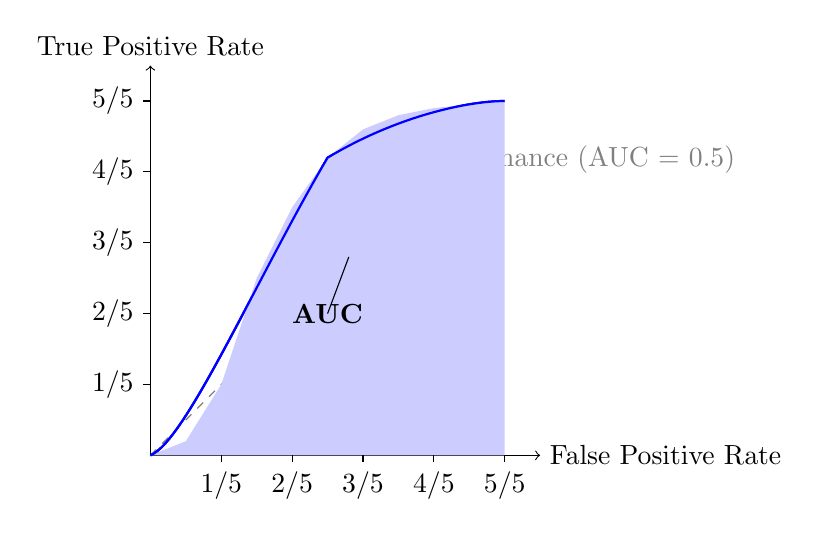
\begin{tikzpicture}[scale=0.9]
    % Axes
    \draw[->] (0,0) -- (5.5,0) node[right] {False Positive Rate};
    \draw[->] (0,0) -- (0,5.5) node[above] {True Positive Rate};
    
    % Chance diagonal
    \draw[dashed, gray] (0,0) -- (5,5) node[pos=0.9, below right] {Chance (AUC = 0.5)};
    
    % ROC curve (concave, typical good classifier)
    \draw[thick, blue] (0,0) .. controls (0.5,0.2) and (1.5,2.5) .. (2.5,4.2) .. controls (3.5,4.8) and (4.5,5) .. (5,5);
    
    % Shaded area under ROC curve (AUC)
    \fill[blue!20] (0,0) -- (0.5,0.2) -- (1,1) -- (1.5,2.5) -- (2,3.5) -- (2.5,4.2) -- (3,4.6) -- (3.5,4.8) -- (4,4.9) -- (4.5,4.95) -- (5,5) -- (5,0) -- cycle;
    
    % Redraw curve on top of fill
    \draw[thick, blue] (0,0) .. controls (0.5,0.2) and (1.5,2.5) .. (2.5,4.2) .. controls (3.5,4.8) and (4.5,5) .. (5,5);
    
    % Labels
    \node at (2.5,2) {\textbf{AUC}};
    \draw (2.5,2) -- (2.8,2.8);
    
    % Tick marks
    \foreach \x in {1,2,3,4,5} {
        \draw (\x,0) -- (\x,-0.1) node[below] {\x/5};
        \draw (0,\x) -- (-0.1,\x) node[left] {\x/5};
    }
\end{tikzpicture}
\caption{An ROC curve. The blue curve shows TPR vs FPR as the classifier threshold is swept. The shaded area under the curve is the AUC. The dashed diagonal represents chance performance (AUC = 0.5).}
\end{figure}

\subsection{Logistic Regression as a ``Linear Probe''}

\subsubsection{What Is Logistic Regression?}

\textbf{Logistic regression} is a simple statistical model that finds a \textbf{flat hyperplane} in a high-dimensional space to separate two groups. In 2D, a hyperplane is a straight line; in 3D, it is a flat plane; in many dimensions, it is still ``flat''---no curves, no bends. The model learns weights such that one side of the hyperplane tends to have positives and the other side negatives.

\subsubsection{Why ``Linear''?}

``Linear'' means the decision boundary is a straight line (in 2D) or a flat hyperplane (in higher dimensions). The model cannot draw curved boundaries. If the two groups are arranged in a circle versus everything inside, a linear classifier would struggle. If they are separated by a straight cut, a linear classifier excels.

\subsubsection{Using It as a Probe}

In our paper, we do \emph{not} use logistic regression to build a new lens finder. We use it as a \textbf{diagnostic probe}: we take the internal representations (embeddings) that the CNN produces for each image and ask, ``Can a simple linear classifier separate real lenses from parametric injections using just these embeddings?''

If the answer is yes---if logistic regression achieves AUC near 1.0---then the two groups are \textbf{trivially separable} in that feature space. The CNN's internal representation makes it easy to tell them apart with a straight cut. That means the parametric injections do \emph{not} look like real lenses to the CNN; they occupy a different region of feature space.

If the answer is no---if logistic regression gets AUC near 0.5---then the two groups overlap. The CNN cannot easily tell them apart with a linear boundary, which suggests the injections may be more realistic.

It is called a ``probe'' because we are \emph{probing} what the CNN has learned, not training a new classifier from scratch. The CNN is already trained; we are just inspecting its feature space.

\subsection{Cross-Validation (k-Fold)}

\subsubsection{Why Not Test on Training Data?}

If we train a model on a dataset and then evaluate it on the \emph{same} data, we get an overly optimistic result. The model has already ``seen'' those examples and can memorize them. This is called \textbf{overfitting}. To get an honest estimate of performance, we must test on data the model has never seen.

\subsubsection{The k-Fold Procedure}

\textbf{k-fold cross-validation} splits the data into $k$ equal parts (folds). We do $k$ rounds:

\begin{enumerate}
    \item Round 1: Train on folds 2, 3, 4, 5; test on fold 1.
    \item Round 2: Train on folds 1, 3, 4, 5; test on fold 2.
    \item Round 3: Train on folds 1, 2, 4, 5; test on fold 3.
    \item Round 4: Train on folds 1, 2, 3, 5; test on fold 4.
    \item Round 5: Train on folds 1, 2, 3, 4; test on fold 5.
\end{enumerate}

Each fold serves as the test set exactly once. We rotate through all folds so every data point is used for testing once. We report the \textbf{mean} and \textbf{standard deviation} of the metric (e.g., AUC) across the $k$ folds. The mean gives our best estimate; the standard deviation tells us how stable the result is.

\subsubsection{In Our Paper}

We use 5-fold cross-validation with 112 real lens embeddings and 500 parametric injection embeddings. Each fold has roughly 90\% for training and 10\% for testing. We report mean AUC and its standard deviation across the 5 folds. This ensures our linear probe result is not due to a lucky split of the data.

\begin{figure}[htbp]
\centering
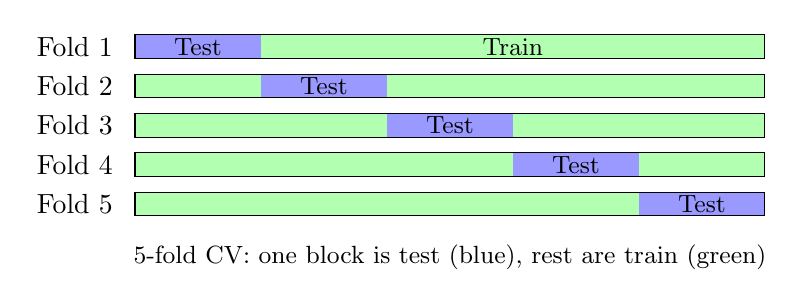
\begin{tikzpicture}[x=0.8cm, y=0.5cm]
    % Fold 1: block 1 test, blocks 2-5 train
    \fill[blue!40] (0,5) rectangle (2,5.6);
    \fill[green!30] (2,5) rectangle (10,5.6);
    \draw (0,5) rectangle (10,5.6);
    \node[left] at (-0.2, 5.3) {Fold 1};
    \node at (1, 5.3) {\small Test};
    \node at (6, 5.3) {\small Train};
    % Fold 2: block 2 test
    \fill[green!30] (0,4) rectangle (2,4.6);
    \fill[blue!40] (2,4) rectangle (4,4.6);
    \fill[green!30] (4,4) rectangle (10,4.6);
    \draw (0,4) rectangle (10,4.6);
    \node[left] at (-0.2, 4.3) {Fold 2};
    \node at (3, 4.3) {\small Test};
    % Fold 3: block 3 test
    \fill[green!30] (0,3) rectangle (4,3.6);
    \fill[blue!40] (4,3) rectangle (6,3.6);
    \fill[green!30] (6,3) rectangle (10,3.6);
    \draw (0,3) rectangle (10,3.6);
    \node[left] at (-0.2, 3.3) {Fold 3};
    \node at (5, 3.3) {\small Test};
    % Fold 4: block 4 test
    \fill[green!30] (0,2) rectangle (6,2.6);
    \fill[blue!40] (6,2) rectangle (8,2.6);
    \fill[green!30] (8,2) rectangle (10,2.6);
    \draw (0,2) rectangle (10,2.6);
    \node[left] at (-0.2, 2.3) {Fold 4};
    \node at (7, 2.3) {\small Test};
    % Fold 5: block 5 test
    \fill[green!30] (0,1) rectangle (8,1.6);
    \fill[blue!40] (8,1) rectangle (10,1.6);
    \draw (0,1) rectangle (10,1.6);
    \node[left] at (-0.2, 1.3) {Fold 5};
    \node at (9, 1.3) {\small Test};
    \node[below, font=\small] at (5, 0.5) {5-fold CV: one block is test (blue), rest are train (green)};
\end{tikzpicture}
\caption{Schematic of 5-fold cross-validation. Each horizontal bar represents one round. The blue block is the test set; the green blocks are the training set. The test block rotates across the five rounds.}
\end{figure}

\subsection{Confidence Intervals}

A point estimate (e.g., ``recall is 80\%'') is useful, but we also want to know how precise it is. \textbf{Confidence intervals} give a range of plausible values. We use two types.

\subsubsection{Wilson Score Interval for Proportions}

When we estimate a proportion (e.g., recall $= \frac{\text{recovered}}{\text{injected}}$), the naive formula $\hat{p} \pm z \sqrt{\hat{p}(1-\hat{p})/n}$ works poorly for small samples or proportions near 0 or 1. The \textbf{Wilson score interval} is a formula that accounts for this and produces more reliable intervals. It is what we use for recall and other proportions in the paper.

\subsubsection{Bootstrap Confidence Intervals for AUC}

For AUC, we use the \textbf{bootstrap}:

\begin{enumerate}
    \item Resample the data \emph{with replacement} to get a new dataset of the same size (some points appear multiple times, some not at all).
    \item Compute AUC on this resampled dataset.
    \item Repeat many times (e.g., 1000 or 10,000).
    \item The bootstrap distribution of AUC approximates the sampling distribution. A 95\% confidence interval is the 2.5th to 97.5th percentile of this distribution.
\end{enumerate}

The bootstrap makes minimal assumptions about the underlying distribution and is widely used for complex statistics like AUC.

\subsection{Permutation Tests}

\subsubsection{The Logic}

\textbf{Permutation testing} answers: ``If there were really no difference between the two groups, how often would we see a result as extreme as ours by chance?'' The key idea: \emph{if the groups are the same, then shuffling the labels should not change the result}. We can simulate this by randomly reassigning ``lens'' and ``non-lens'' labels and recomputing our statistic (e.g., AUC) each time.

\subsubsection{The Procedure}

\begin{enumerate}
    \item Compute the observed test statistic (e.g., AUC $= 0.997$ for separating real lenses from parametric injections).
    \item Shuffle the labels: randomly swap ``lens'' and ``injection'' among the 612 embeddings. The scores stay attached to each embedding; only the labels change.
    \item Train the linear probe on the shuffled data and compute AUC.
    \item Repeat step 2--3 many times (e.g., 1000 permutations).
    \item The \textbf{p-value} is the fraction of permutations where the permuted AUC $\geq$ observed AUC (plus a small correction, e.g., add 1 to numerator and denominator, to avoid p-value $= 0$).
\end{enumerate}

If the observed AUC (0.997) is far to the right of the permutation distribution (centered near 0.5), then very few---or zero---permutations beat it. The p-value is tiny. We conclude that the separation is statistically significant: it is extremely unlikely to arise by chance if the two groups were the same.

\subsubsection{Why Permutation Tests Are Powerful}

Permutation tests make \textbf{no assumptions} about the distribution of the data. They do not require normality or any parametric model. They are exact (or nearly exact) for the null hypothesis that the labels are exchangeable. They are ideal when we have a complex statistic like AUC and want a nonparametric test.

\begin{figure}[htbp]
\centering
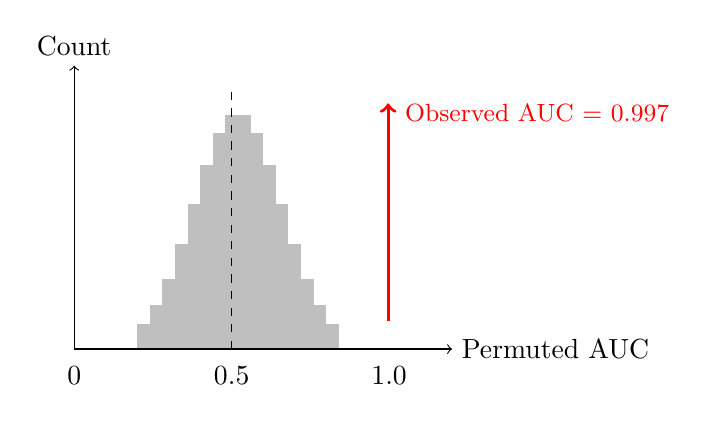
\begin{tikzpicture}[x=4cm, y=1.2cm]
    % Histogram bars (permutation distribution centered at 0.5)
    \foreach \i in {0,...,15} {
        \pgfmathsetmacro{\x}{0.2 + \i*0.04}
        \pgfmathsetmacro{\h}{2.5*exp(-25*(\x-0.5)*(\x-0.5))}
        \fill[gray!50] (\x, 0) rectangle (\x+0.04, \h);
    }
    % Axes
    \draw[->] (0,0) -- (1.2,0) node[right] {Permuted AUC};
    \draw[->] (0,0) -- (0,3) node[above] {Count};
    % Red arrow at observed AUC (0.997 off scale, in margin)
    \draw[red, very thick, ->] (0.997, 0.3) -- (0.997, 2.6);
    \node[red, right, font=\small] at (1.02, 2.5) {Observed AUC = 0.997};
    % Vertical dashed line at 0.5
    \draw[dashed] (0.5, 0) -- (0.5, 2.8);
    \node[below] at (0.5, -0.08) {0.5};
    \node[below] at (0, -0.08) {0};
    \node[below] at (1.0, -0.08) {1.0};
\end{tikzpicture}
\caption{Permutation test. The gray histogram shows the distribution of AUC when labels are randomly shuffled (centered near 0.5). The red arrow marks our observed AUC (0.997). Almost no permutations reach that value, so the p-value is extremely small.}
\end{figure}

\subsection{Fr\'echet Distance}

The \textbf{Fr\'echet distance} (sometimes called the Fr\'echet Inception Distance in machine learning) measures how different two probability distributions are in high-dimensional space. Given two sets of points (e.g., embeddings from real lenses vs parametric injections), we compute the mean and covariance matrix of each set. The Fr\'echet distance combines the difference between the means and the difference between the covariances into a single number.

\textbf{Larger Fr\'echet distance} = the two distributions are more different. Smaller = more similar. It is useful for comparing whether two sets of embeddings occupy similar regions of feature space.

\textbf{Caveat}: When the sample size is smaller than the dimensionality (e.g., 112 embeddings in a 512-dimensional space), the covariance matrix becomes \textbf{singular} (not invertible). The Fr\'echet distance formula breaks down. It is unreliable in such cases, so we must be careful when interpreting it for small datasets.

\subsection{Understanding p-Values}

A \textbf{p-value} answers: ``If the null hypothesis were true (e.g., there is no difference between groups), what is the probability of observing a result as extreme as ours---or more extreme---just by chance?''

\textbf{What p-values mean}: A small p-value (e.g., $p < 0.05$) means that such an extreme result would be rare if the null were true. So we have evidence against the null; we may reject it.

\textbf{What p-values do NOT mean}: A p-value is \emph{not} the probability that the null hypothesis is true. It is \emph{not} the probability that our result is a fluke. It assumes the null is true and asks how often we would see data this weird. This is a subtle but crucial distinction.

\subsection{Comparing Two Proportions: The Two-Proportion z-Test}

When we compare two percentages (e.g., completeness of 5.18\% vs 3.79\%), we use a \textbf{two-proportion z-test}. We compute a z-statistic based on the difference between the two proportions and their combined standard error. Under the null hypothesis that the two proportions are equal, this z-statistic follows (approximately) a standard normal distribution. We can then compute a p-value.

For example, if we find 5.18\% completeness in one sample and 3.79\% in another, the z-test tells us whether that difference is statistically significant or could easily have arisen by chance.

\subsection{The Sign Test}

When we have \textbf{paired} binary outcomes (e.g., for each of 112 lenses, we have two classifications: ``found by method A'' and ``found by method B''), the \textbf{sign test} compares the two methods. For each pair, we note whether A and B agree or disagree. We count how many times A found a lens when B did not, and vice versa. Under the null that the two methods are equally good, we expect roughly equal numbers in each direction. The sign test uses the binomial distribution to compute how unlikely an imbalance is. It is simple, nonparametric, and does not assume normality.

\bigskip
\noindent\textit{We use these tools throughout the paper: AUC and the linear probe to diagnose injection realism, cross-validation for robust estimates, permutation tests for significance, and confidence intervals and proportion tests to compare completeness and recall across methods.}

\newpage
\section{Chapter 5: The DESI Legacy Imaging Survey}

The images we use for finding strong lenses come from the \textbf{DESI Legacy Imaging Survey}. This section explains what that survey is, what its data look like, and why these choices matter for our analysis.

\subsection{What Is DESI?}

\textbf{DESI} stands for the \textbf{Dark Energy Spectroscopic Instrument}. It is a large spectroscopic survey designed to measure the distances and velocities of tens of millions of galaxies and quasars. Its goal is to map the large-scale structure of the universe and constrain dark energy---the mysterious component causing cosmic acceleration.

DESI needs a catalog of targets to observe: galaxies and quasars with positions, brightnesses, and colors. That catalog comes from \textbf{imaging}---taking pictures of the sky in several bands. DESI does not do its own imaging; it uses data from the \textbf{Legacy Imaging Surveys}, which were specifically designed to support DESI target selection.

\subsection{Data Release 10 (DR10)}

\textbf{DR10} is the \textbf{Data Release 10}---the tenth public release of the Legacy Imaging Survey data. Each release incorporates new observations, improved processing, and refined calibrations. DR10 represents the state of the data at the time of our analysis. It combines imaging from three surveys: the \textbf{Dark Energy Camera Legacy Survey} (DECaLS), the \textbf{Beijing-Arizona Sky Survey} (BASS), and the \textbf{Mayall z-band Legacy Survey} (MzLS). Together they cover the extragalactic sky visible from the northern hemisphere.

\subsection{The Three Optical Bands}

The Legacy Survey observes in three optical bands:

\begin{itemize}
    \item \textbf{g band} (blue-green): Central wavelength $\sim 475$ nm. Sensitive to younger, bluer stellar populations and star-forming regions.
    \item \textbf{r band} (red): Central wavelength $\sim 622$ nm. Often the ``fiducial'' band for morphology; good balance of depth and resolution.
    \item \textbf{z band} (near-infrared): Central wavelength $\sim 913$ nm. Probes redder, older stellar light; less affected by dust extinction.
\end{itemize}

Together, g, r, and z provide \textbf{color} information. The ratio of flux in different bands tells us about stellar populations, dust, and redshift. For strong lenses, the lens galaxy is typically an old, red elliptical, while the background source can be bluer. Color helps distinguish lenses from non-lenses.

\subsection{Pixel Scale: What Does 0.262 Arcsec Mean?}

The \textbf{pixel scale} is 0.262 arcsec per pixel. An \textbf{arcsecond} is $1/3600$ of a degree---a very small angle. The full Moon is about 1800 arcsec across, so one arcsecond is roughly 1/1800 of the Moon's diameter.

At typical lens redshifts ($z \sim 0.3$--0.5), 1 arcsec corresponds to about 3--5 \textbf{kiloparsecs} (kpc). A kiloparsec is about 3260 light-years, so 1 arcsec spans roughly 10,000--16,000 light-years at these distances. That means each pixel (0.262 arcsec) corresponds to about 800--4000 light-years. The pixel scale sets the smallest spatial features we can resolve.

\subsection{Depth: How Faint Can We See?}

\textbf{Depth} describes how faint an object can be and still be detected. Surveys quote \textbf{5-sigma depth}: the magnitude at which a point source is detected with 5-sigma significance (i.e., the signal is 5 times the noise). For the Legacy Survey, typical 5-sigma depths are:

\begin{itemize}
    \item g $\sim 24.7$ mag
    \item r $\sim 23.9$ mag
    \item z $\sim 23.0$ mag
\end{itemize}

Each magnitude step of 1 corresponds to a factor of about 2.5 in brightness (on the logarithmic magnitude scale). So mag 24 is about 2.5 times fainter than mag 23, and about $2.5^4 \approx 40$ times fainter than mag 20. The brightest stars visible to the naked eye are around mag 6. Mag 24 is roughly $2.5^{18} \approx 100$ million times fainter. These depths allow us to detect distant lensed galaxies that would be invisible in shallower surveys.

\subsection{Seeing: Atmospheric Blurring}

\textbf{Seeing} refers to the blurring of images by Earth's atmosphere. Turbulent air cells deflect light, so a point source spreads into a blob. The \textbf{point spread function} (PSF) describes this blur. Its width is often quantified by the \textbf{FWHM} (Full Width at Half Maximum): the diameter of the blob at half its peak brightness.

The median seeing in the r-band is about 1.3 arcsec. That means features smaller than $\sim 1.3$ arcsec are blurred together. Strong lens arcs can be a few arcseconds long, so they are marginally resolved. Better seeing (smaller FWHM) would sharpen the arcs; worse seeing would smear them further.

\subsection{Nanomaggies: The Flux Unit}

The Legacy Survey reports flux in \textbf{nanomaggies}. One nanomaggy corresponds to AB magnitude 22.5. The conversion is:
\begin{equation}
\text{flux}_{\text{nanomaggy}} = 10^{(22.5 - \text{magnitude})/2.5}
\end{equation}
So magnitude 22.5 gives 1 nanomaggy; magnitude 20 gives $10^{1} = 10$ nanomaggies; magnitude 25 gives $10^{-1} = 0.1$ nanomaggies. Working in linear flux (nanomaggies) is convenient for modeling and for combining bands.

\subsection{Cutouts: Our 101$\times$101 Pixel Images}

We do not use full survey images. We extract \textbf{cutouts}: small square regions centered on each galaxy of interest. Our cutouts are 101$\times$101 pixels.

With 0.262 arcsec per pixel, 101 pixels span $101 \times 0.262 \approx 26.5$ arcsec on a side. So each cutout covers about $26.5 \times 26.5$ square arcseconds. This is large enough to capture the lens galaxy, any lensed arcs, and surrounding sky; it is small enough to be computationally manageable and to avoid too much contamination from neighboring objects.

\subsection{Survey Coverage}

The Legacy Imaging Survey covers approximately 14,000 square degrees of sky---about one-third of the entire sky. This is the northern extragalactic sky, avoiding the plane of the Milky Way where dust and stars would contaminate the data. The large area means we have many galaxies to search for lenses, but it also means we rely on automated methods like CNNs to process the data.

\bigskip
\noindent\textit{In summary: We use DR10 cutouts in g, r, and z bands, with 0.262 arcsec pixels, depth to mag $\sim$24, and seeing $\sim$1.3 arcsec. These choices match the real survey conditions under which our CNN was trained and will be applied.}

\newpage
\section{Chapter 6: Prior Work This Paper Builds On}

Our paper did not arise in a vacuum. Several earlier studies laid the groundwork and identified key limitations. This chapter summarizes each contribution and the gap that our work fills.

\subsection{Herle et al.\ (2024): Biases in CNN Detection}

\textbf{Reference:} Herle et al., MNRAS \textbf{534}, 1093 (2024).

Herle and collaborators studied how a CNN lens finder's \textbf{detection probability} depends on lens and source properties. They varied the Einstein radius (a measure of lens strength), the S\'ersic index (a measure of how ``concentrated'' the lens galaxy light is), and the source size. Using \textbf{simulated Euclid-like data}---space-based imaging with higher resolution than ground-based surveys---they trained a CNN and measured its detection rate as a function of these parameters.

\textbf{Key finding:} Detection is \textbf{strongly biased}. The CNN preferentially finds certain types of lenses: those with larger Einstein radii, particular S\'ersic indices, and certain source sizes. Lenses that fall outside these ``sweet spots'' are missed more often. In other words, the CNN has a \textbf{selection function} that is not uniform across lens parameter space.

\textbf{Limitation:} Herle et al.\ worked entirely in simulation. They never compared their simulated lenses to real confirmed lenses. So they demonstrated that the selection function is biased in a simulated world, but they could not say whether those simulated lenses look \emph{realistic} to the CNN. If the simulations are wrong, the inferred bias may not apply to the real universe. Our paper directly addresses that gap by comparing real lenses to simulated injections in the CNN's feature space.

\subsection{Canameras et al.\ (2024, HOLISMOKES XI): Real-Galaxy Sources}

\textbf{Reference:} Canameras et al., A\&A \textbf{692}, A72 (2024)---HOLISMOKES XI.

Canameras and collaborators took a different approach to realism. Instead of using \textbf{parametric models} (e.g., S\'ersic profiles) for the background source galaxies, they used \textbf{real galaxy images} from the \textbf{Hubble Ultra Deep Field} (HUDF). They ``injected'' these real-galaxy sources into \textbf{Hyper Suprime-Cam} (HSC) survey imaging---a different telescope and survey from the Legacy Survey, but also ground-based optical imaging.

\textbf{Key contribution:} They explicitly noted that \textbf{S\'ersic profiles are inadequate} for modeling real sources. Real galaxies have irregular shapes, spiral arms, clumps, and asymmetric structure. A smooth S\'ersic ellipse cannot capture that. By using real HUDF galaxies, they bypassed the parametric limitation entirely.

\textbf{Limitation:} They did \emph{not} quantify how different parametric and real injections look in the CNN's internal representation. Their observation was qualitative: real galaxies look more realistic. Our paper provides a \textbf{quantitative} diagnostic: we measure the linear probe AUC between real lenses and parametric injections in embedding space. We show that the difference is large (AUC $\approx$ 0.997) and statistically significant. We also propose this as a tool the community can use to evaluate any injection scheme.

\subsection{Collett \& Cunnington (2022): The Injection-Recovery Framework}

\textbf{Reference:} Collett \& Cunnington, MNRAS \textbf{516}, 1808 (2022).

Collett and Cunnington established the \textbf{injection-recovery framework} for calibrating CNN lens finder selection functions. The idea: simulate lenses by injecting synthetic lensed sources into real survey images, run the CNN on the result, and measure the recovery fraction. This gives an empirically calibrated completeness curve: at each lens parameter value, what fraction of injected lenses does the CNN find?

They used \textbf{parametric models}: a singular isothermal ellipse (SIE) for the lens and a S\'ersic profile for the source. Their methodology is foundational---it is the standard approach in the field. Our paper builds on this framework but asks: do parametric injections produce the same recovery statistics as real lenses would? If not, the calibration may be wrong. Our linear probe provides a way to test that.

\subsection{Huang et al.\ (2020): The DECaLS Lens Catalog}

\textbf{Reference:} Huang et al., ApJ \textbf{894}, 78 (2020).

Huang and collaborators applied a \textbf{ResNet} CNN to find strong lens candidates in the DECaLS survey---a predecessor to and component of the Legacy Survey DR10. They produced a large catalog of candidates and released it to the community.

\textbf{Limitation:} They did \emph{not} perform injection-recovery or completeness analysis. They focused on finding candidates, not on calibrating the selection function. Our work assumes such a catalog exists (or could exist) and asks: when we calibrate it with injections, are those injections realistic enough?

\subsection{The Gap Our Paper Fills}

No prior work had done all of the following:

\begin{enumerate}
    \item \textbf{Directly measured} how different real lenses look from parametric injections in CNN feature space. Herle et al.\ used simulation only; Canameras et al.\ used real galaxies but did not quantify the difference in embedding space.
    \item \textbf{Performed a controlled experiment} to diagnose the cause. We compare real lenses to parametric injections, and real lenses to real-galaxy injections, in the same embedding space. We show that the problem is the source model (parametric vs.\ real), not the lens or the pipeline.
    \item \textbf{Proposed a quantitative diagnostic tool}---the linear probe AUC---that the community can use to evaluate any injection scheme. Before our paper, there was no standard way to ask: ``Do my injections look like real lenses to this CNN?'' Now there is.
\end{enumerate}

Our paper thus bridges the gap between simulation-based calibration (Collett \& Cunnington, Herle et al.) and the qualitative recognition that real galaxies matter (Canameras et al.). We provide a concrete, implementable test: if the linear probe AUC between real lenses and your injections is near 1.0, your injections are not realistic. If it is near 0.5, they may be. This is a step toward more reliable completeness calibration for CNN lens finders.


% ====================================================================
% PART II
% ====================================================================
% LaTeX body content for Part II, Chapters 7-9
% Research Companion Guide - CNN Strong Gravitational Lens Finding
% Audience: high school student who led the research

\part{What We Did}

\section{Chapter 7: Our Data and Model}

This chapter describes the ingredients we used to train our CNN lens finder: the images, the labels, and the training procedure. Understanding these choices is essential for interpreting the results we present later.

\subsection{The Training Set: 451,681 Cutouts}

We trained our CNN on a large set of small square images called \textbf{cutouts}. Each cutout is a 101$\times$101 pixel region of the sky centered on a galaxy. In total, we had 451,681 cutouts, divided into:
\begin{itemize}
    \item \textbf{316,100} for training (the data the model learns from)
    \item \textbf{135,581} for validation (the data we use to check how well the model generalizes, without ever training on it)
\end{itemize}
The validation set lets us measure performance honestly---if we evaluated on the training data, the model might have ``memorized'' specific examples rather than learned general lens-finding rules.

\subsection{Positive Examples: Tier-A and Tier-B Lenses}

Our positive examples---images that show a strong lens---come in two tiers based on how certain we are that they are real lenses.

\subsubsection{Tier-A Positives: Spectroscopically Confirmed}

\textbf{Tier-A} lenses are the gold standard. We have 277 in training and 112 in validation (389 total). These are \textbf{spectroscopically confirmed} strong lenses.

\textbf{What does ``spectroscopically confirmed'' mean?} When astronomers want to prove that a lens is real, they measure the \textbf{redshift} of the light from different parts of the image. Redshift is a measure of how much the light has been stretched by the expansion of the universe---objects farther away have higher redshift. A strong lens produces multiple images of the same background galaxy. When you split the light from each image into a \textbf{spectrum} (a rainbow showing how much light arrives at each wavelength), you can measure the redshift. If you find \emph{two different redshifts} at the same position on the sky---one from the foreground lens galaxy and one from the background source---you have proof that lensing is occurring. The lens galaxy is in front, bending light from the more distant source. That is spectroscopic confirmation.

Tier-A lenses are our most reliable labels. We use them for our headline recall metric: how well does the CNN find lenses that we \emph{know} are real?

\subsubsection{Tier-B Positives: Visual Candidates}

\textbf{Tier-B} lenses are visually identified candidates: 3,079 in training and 1,320 in validation. These were flagged by citizen scientists (volunteers classifying galaxies) and by expert astronomers inspecting images. They look like lenses---they have arc-like features, multiple images, or other lens signatures---but they have not been spectroscopically confirmed. We estimate that roughly 10\% of Tier-B may \emph{not} actually be lenses. This is called \textbf{label noise}: some of our ``positive'' training examples might be false. We chose not to overweight these positives in our loss function precisely because of this uncertainty; giving them too much weight could cause the model to overfit to impostors.

\subsection{Negative Examples: Non-Lens Galaxies}

The negatives---images that do \emph{not} show a strong lens---number approximately 447,000. These are ordinary galaxies from the survey catalog, selected to span the full range of galaxy types: ellipticals, spirals, irregulars, bright and faint. Including diverse negatives ensures the CNN learns to distinguish lenses from all kinds of non-lenses, not just from one narrow type.

\subsection{Class Imbalance: One Lens per 93 Non-Lenses}

The ratio of positives to negatives is about 1:93. For every lens in our data, there are roughly 93 non-lenses. This might seem unfair---why so few lenses?---but it reflects reality. Strong lenses are rare in the universe. In a wide-area survey, you might find one lens per several thousand galaxies. Training with a 1:93 ratio matches the \textbf{class imbalance} the model will face when applied to real survey data. If we had artificially balanced the classes (e.g., 50\% lenses), the CNN might learn behaviors that do not generalize to the true rarity of lenses in the field.

\subsection{Spatial Integrity: Why HEALPix Matters}

A subtle but crucial concern: could the model cheat by memorizing specific regions of the sky? If a lens in the validation set lay in the same patch of sky as many training examples, the CNN might have learned that ``this patch = lens'' without understanding what a lens looks like. To prevent this, we used \textbf{HEALPix} to enforce \textbf{spatial integrity}.

\textbf{HEALPix} (Hierarchical Equal Area isoLatitude Pixelization) is a scheme that divides the entire sky into equal-area pixels. We used NSIDE$=128$, which creates roughly 786,000 pixels. Each point on the sky belongs to exactly one HEALPix pixel. The key rule: \emph{training Tier-A lenses and validation Tier-A lenses occupy completely separate HEALPix pixels}. We have 274 unique training pixels and 112 unique validation pixels, with \textbf{zero overlap}. No validation lens shares a sky pixel with any training lens. This guarantees that when we evaluate recall on the 112 validation lenses, we are testing on genuinely new sky---the model has never seen those regions during training. It cannot have memorized them.

\subsection{Two-Phase Training}

We trained the CNN in two phases.

\textbf{Phase 1:} We started from weights pretrained on \textbf{ImageNet} (a large dataset of everyday images: cats, cars, landscapes). This transfer learning gives the model a head start on recognizing shapes and textures. We trained for 160 epochs. The best validation AUC (0.9915) was reached at epoch 19. We saved those weights.

\textbf{Phase 2:} We loaded the epoch-19 weights and fine-tuned for 60 additional epochs with a \textbf{cosine decay} learning rate schedule (the learning rate smoothly decreases over time). This produced our final model, with validation AUC 0.9921. The modest gain from Phase 2 (0.9915 $\to$ 0.9921) suggests the model was already performing well; fine-tuning refined it slightly.

\subsection{Augmentation: Flip and Rotate}

During training, we applied \textbf{geometric augmentation} to \emph{all} cutouts---both positives and negatives. Each time an image was fed to the model, we randomly:
\begin{itemize}
    \item Flipped it horizontally (50\% probability)
    \item Flipped it vertically (50\% probability)
    \item Rotated it by 0, 90, 180, or 270 degrees (chosen uniformly)
\end{itemize}
These transformations do not change the content: a lens flipped sideways is still a lens. They help the model learn that lenses look like lenses regardless of orientation, reducing overfitting.

We did \emph{not} apply noise or color augmentation. This choice is important for a later experiment (Chapter 10): when we test whether adding Poisson noise to injections improves detection, we are testing a distribution shift the model has never seen during training. The model was trained on real survey noise, not on artificially noised parametric arcs.

\subsection{Preprocessing: \texttt{raw\_robust} Mode}

Before feeding an image to the CNN, we \textbf{preprocess} it. We use a mode called \texttt{raw\_robust}. For each band (g, r, z) independently:

\begin{enumerate}
    \item \textbf{Compute the median} of pixels in an \textbf{annulus}---a ring-shaped region around the center of the image, between inner radius 20 pixels and outer radius 32 pixels. This region is dominated by sky (background) rather than the galaxy or arc. The median estimates the sky level.
    \item \textbf{Subtract this median} from every pixel. This removes the sky background. Sky-dominated pixels now sit near zero.
    \item \textbf{Divide by the MAD} (median absolute deviation) of the same annulus. MAD measures the typical spread of pixel values; it is a robust estimate of the noise level. Dividing by MAD \textbf{normalizes} the image so that noise has unit scale. Galaxy and arc features appear as positive excursions of several units.
    \item \textbf{Clip} pixel values to the range $[-10, +10]$. Very bright or very dark pixels (e.g., saturated stars) are capped, preventing outliers from dominating.
\end{enumerate}

After preprocessing, sky-dominated pixels sit near zero with unit noise scale. Galaxy and lensed-arc features appear as positive values. The CNN sees images in this normalized space, which makes learning more stable and invariant to overall brightness and depth variations across the survey.

\bigskip
\noindent\textit{In summary: We trained on 451,681 cutouts with 1:93 class imbalance, using Tier-A and Tier-B positives and diverse negatives. HEALPix ensured no spatial overlap between training and validation Tier-A lenses. Two-phase training and geometric augmentation produced a model with AUC 0.9921. Preprocessing in raw\_robust mode normalized each band by sky median and MAD.}

\newpage
\section{Chapter 8: The Injection Pipeline}

To test whether our CNN can detect synthetic lenses, we need a way to create them. This chapter explains our \textbf{injection pipeline}: the procedure we use to generate synthetic lensed arcs and add them to real galaxy images. Understanding the pipeline is essential for interpreting why our injections look different from real lenses to the CNN.

\subsection{The Goal}

The goal of the injection pipeline is to create \textbf{synthetic lensed arcs}---fake lensed galaxies---and add them to real survey images. We then run the CNN on the resulting images and ask: does it detect them? If we inject 100 synthetic lenses and the CNN finds 50 of them, we say the \textbf{completeness} at those parameter values is 50\%. By varying the injection parameters (lens strength, source brightness, etc.), we build a completeness map: at each configuration, what fraction of injections does the CNN recover? This calibration tells us how ``detectable'' different types of lenses are to our model.

The catch: if our synthetic lenses do not look like real lenses to the CNN, the completeness map we measure will not reflect what would happen with real lenses. This chapter describes how we build the injections; the next chapter reveals the gap.

\subsection{The Lens Model: Singular Isothermal Ellipsoid (SIE)}

The \textbf{lens} is the foreground galaxy whose gravity bends the light. We model its mass distribution as a \textbf{Singular Isothermal Ellipsoid} (SIE).

\textbf{What does that mean?} ``Isothermal'' refers to a gas at constant temperature. In such a gas, the velocity dispersion (how fast particles move) is constant with radius. Astrophysicists use this as a simple approximation for the mass distribution of elliptical galaxies: the ``temperature'' is a stand-in for the velocity dispersion of stars. The mass density falls off as $1/r^2$, producing a characteristic deflection of light. ``Ellipsoid'' means the mass distribution is elliptical (elongated), not perfectly spherical. ``Singular'' means the density goes to infinity at the center---a mathematical idealization that works well for unresolved central regions.

The key SIE parameters:
\begin{itemize}
    \item \textbf{Einstein radius} $\theta_E$: Controls the size of the lensing effect. Larger $\theta_E$ means stronger lensing and larger arcs. We use $\theta_E$ from 0.5 to 3.0 arcsec in our grid (0.25 arcsec steps).
    \item \textbf{Axis ratio} $q_{\mathrm{lens}}$: How elongated the mass distribution is. $q = 1$ is a circle; $q = 0.5$ is quite flattened. We draw $q$ from 0.5 to 1.0.
    \item \textbf{Position angle}: The orientation of the ellipse on the sky.
    \item \textbf{External shear}: Tidal gravitational effects from nearby galaxies. We add small random shear components to make the lens environment more realistic.
\end{itemize}

\subsection{The Source Model: S\'ersic Profile}

The \textbf{source} is the background galaxy whose light gets lensed. We model it as a \textbf{S\'ersic profile}.

A S\'ersic profile is a mathematical formula that describes how a galaxy's brightness falls off from its center to its edge. The \textbf{S\'ersic index} $n$ controls the shape:
\begin{itemize}
    \item $n = 1$: Exponential profile---typical of disk galaxies (spirals).
    \item $n = 4$: De Vaucouleurs profile---typical of elliptical galaxies.
    \item We use $n$ from 0.5 to 2.0, favoring disk-like and intermediate morphologies.
\end{itemize}

Other source parameters:
\begin{itemize}
    \item \textbf{Magnitude} $m_r$: Brightness in the r-band. For bright-arc tests we use 18--26; for the main grid we use 23--26.
    \item \textbf{Effective radius} $R_e$: The half-light radius---the radius containing half the total light. We use 0.15--0.50 arcsec.
    \item \textbf{Colors} $g{-}r$ and $r{-}z$: Calibrated from real lens colors (observer-frame, K-corrected) to match the typical colors of lensed sources at redshift $z \sim 1$--3.
\end{itemize}

\subsubsection{Why S\'ersic Is ``Too Smooth''}

Real galaxies are messy. They have clumps (regions of intense star formation), spiral arms, dust lanes, and irregular structure. A S\'ersic profile is a perfectly smooth mathematical curve. When you lens a S\'ersic source, you get smooth, featureless arcs---elegant curves with no internal structure. Real lensed galaxies produce arcs with knots, bends, and internal detail. This smoothness is one reason our injections may look ``wrong'' to the CNN: real arcs have texture that S\'ersic arcs lack.

\subsection{Source Position: $\beta_{\mathrm{frac}}$}

The \textbf{source position} relative to the lens center matters enormously. We parameterize it as $\beta_{\mathrm{frac}} = \beta / \theta_E$: the offset in units of the Einstein radius.

\begin{itemize}
    \item \textbf{Low} $\beta_{\mathrm{frac}}$ (0.1--0.4): The source sits near the \textbf{caustic}---the region in the source plane where lensing produces dramatic, extended \textbf{tangential arcs}. These are the classic ``banana'' shapes that scream ``lens!''
    \item \textbf{High} $\beta_{\mathrm{frac}}$ ($> 0.5$): The source is farther from the caustic. You get widely separated \textbf{multiple images} (e.g., two or four distinct blobs) that look less like the classic arc morphology.
\end{itemize}

We favor the low-$\beta_{\mathrm{frac}}$ range for our bright-arc experiments because it produces the most lens-like morphologies. The full grid uses the same prior.

\subsection{Ray-Tracing: From Source to Image}

To render the lensed arc, we use \textbf{ray-tracing}. For each pixel in the \textbf{image plane} (what the telescope sees), we trace a light ray backwards through the lens equation to find where it originated in the \textbf{source plane}. We then evaluate the source brightness at that position. This tells us how much light from the source arrived at that image pixel.

We do this on a \textbf{4$\times$ oversampled} grid: 404$\times$404 sub-pixels instead of 101$\times$101. This improves accuracy when the lensed arc has sharp features. After computing the source flux at each sub-pixel, we average down to the native 101$\times$101 resolution.

\subsection{PSF Convolution}

Real telescopes blur images. The \textbf{point spread function} (PSF) describes how a point source (a star) appears as a fuzzy blob. We \textbf{convolve} our rendered arc with a Gaussian PSF that matches the observing conditions of each \textbf{host cutout}---the real galaxy image we inject onto. Different parts of the survey have different seeing (atmospheric blur), so we use the appropriate PSF for each host. Convolution ensures our synthetic arc has the same blur as real objects in that region of the sky.

\subsection{Flux Calibration}

Gravitational lensing conserves \textbf{surface brightness} but amplifies total flux: the lensed image is brighter than the unlensed source because we see more of it (multiple images, extended arcs). We normalize the source profile so that the total flux in the image plane equals the magnification times the unlensed flux. This ensures \textbf{energy conservation}: we are not creating or destroying light, only redistributing it as lensing would.

\subsection{Host Galaxies}

We do not inject onto blank sky. We inject onto \textbf{real survey cutouts} of non-lens galaxies. This ensures that our synthetic lenses sit on realistic backgrounds---galaxy light, sky noise, and survey artifacts---just like real lenses do. The host is drawn from our negative catalog, matching the desired Einstein radius, PSF, and depth for each grid cell.

Critically, we add the injected arc flux \textbf{in nanomaggy space} (linear flux units) \textbf{before} preprocessing. So the injection undergoes the same median subtraction and MAD division as every other feature in the image. The synthetic arc experiences the same normalization as real lensed arcs. This keeps the comparison fair.

\subsection{The Pipeline in One Picture}

\begin{figure}[htbp]
\centering
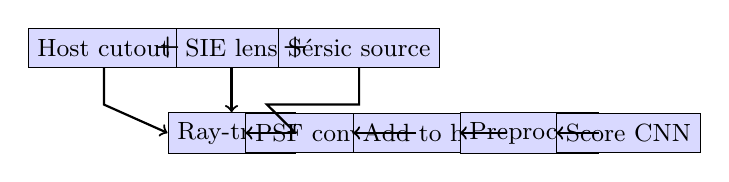
\begin{tikzpicture}[scale=0.9,
    box/.style={rectangle, draw, fill=blue!15, minimum height=0.5cm, minimum width=1.1cm, font=\small}
]
    % Row 1: Inputs
    \node[box] (host) at (0,1.2) {Host cutout};
    \node[box] (sie) at (1.8,1.2) {SIE lens};
    \node[box] (sersic) at (3.6,1.2) {S\'ersic source};
    \node at (0.9,1.2) {\textbf{+}};
    \node at (2.7,1.2) {\textbf{+}};
    
    % Row 2: Process
    \node[box] (raytrace) at (1.8,0) {Ray-trace};
    \node[box] (psf) at (3.2,0) {PSF convolve};
    \node[box] (add) at (4.6,0) {Add to host};
    \node[box] (preproc) at (6.0,0) {Preprocess};
    \node[box] (cnn) at (7.4,0) {Score CNN};
    
    % Arrows from inputs to raytrace
    \draw[->, thick] (host.south) -- (0,0.4) -- (raytrace.west);
    \draw[->, thick] (sie.south) -- (raytrace.north);
    \draw[->, thick] (sersic.south) -- (3.6,0.4) -- (2.3,0.4) -- (raytrace.east);
    
    % Arrows through pipeline
    \draw[->, thick] (raytrace) -- (psf);
    \draw[->, thick] (psf) -- (add);
    \draw[->, thick] (add) -- (preproc);
    \draw[->, thick] (preproc) -- (cnn);
\end{tikzpicture}
\caption{The injection pipeline. We combine a host cutout, an SIE lens model, and a S\'ersic source. Ray-tracing produces the lensed arc; we convolve with the PSF, add to the host in nanomaggy space, preprocess, and score with the CNN.}
\end{figure}

\subsection{Summary}

The injection pipeline produces synthetic lensed arcs using an SIE lens and a S\'ersic source. Ray-tracing, PSF convolution, and flux calibration create realistic-looking arcs in image space. We add them to real host cutouts before preprocessing and pass the result through our CNN. The pipeline is standard in the field---the same general approach used by Collett \& Cunnington and others. The question our paper asks is: do these parametric injections produce the same detection statistics as real lenses? The answer, as we will see, is no.

\bigskip
\noindent\textit{In summary: The injection pipeline combines an SIE lens, a S\'ersic source, and ray-tracing to generate synthetic lensed arcs. We convolve with a survey-matched PSF, add to real host cutouts in nanomaggy space, preprocess, and score with the CNN. S\'ersic sources are smooth and lack the internal structure of real lensed galaxies.}

\newpage
\section{Chapter 9: Results---The Gap}

This chapter presents the main results of our paper: how well the CNN finds real lenses, how well it finds our synthetic injections, and--- crucially---the large gap between the two. We then describe the key diagnostic that reveals why: the linear probe experiment.

\subsection{Real Lens Performance}

On the 112 Tier-A validation lenses, our CNN achieves \textbf{89.3\% recall} at a detection threshold of $p > 0.3$. That means we correctly identify 100 out of 112 spectroscopically confirmed lenses (100/112 $\approx$ 0.893). The 95\% Wilson confidence interval is [82.6\%, 94.0\%]: we are 95\% confident the true recall lies in that range.

\textbf{Twelve lenses are missed} at this threshold. Understanding why---host morphology, Einstein radius, depth, seeing---is the subject of ongoing analysis. For the lenses we do find, the median CNN score is \textbf{0.995}: they cluster at the very high end of the score distribution. The model is confident about real lenses.

\subsection{Injection Completeness}

When we run our injection-recovery experiment over the full parameter grid (Einstein radius 0.5--3.0 arcsec, source magnitude 23--26, varying PSF and depth), we inject 110,000 synthetic lenses. At $p > 0.3$, only \textbf{5.18\%} are detected---5,697 out of 110,000. This is the \textbf{marginal completeness}: the fraction of all injections, averaged over the grid, that the CNN finds.

Most injections in this grid are faint. Source magnitudes 23--26 produce lensed arcs that are often at the limit of detectability. It is no surprise that the overall detection rate is low. The grid is dominated by hard configurations. So the raw comparison---89.3\% real recall vs.\ 5.18\% injection completeness---is not entirely fair. The injection grid includes many genuinely difficult cases that no method would find.

\subsection{The Brightness-Matched Comparison}

To make a fairer comparison, we restrict to \textbf{bright injections}: source magnitude 18--22, which produce lensed arcs at approximately magnitude 16--21 (brighter than most grid injections). We also restrict to low $\beta_{\mathrm{frac}}$ so the arcs are prominent.

Even with these favorable conditions, detection rates are only \textbf{29--39\%}---still a factor of 2--3 below the 89.3\% Tier-A recall. So the gap is not just due to the inclusion of faint injections. When we make injections as bright as (or brighter than) typical confirmed lenses, the CNN still misses most of them. Something else is going on.

\subsection{The Linear Probe: The Paper's Key Diagnostic}

The \textbf{linear probe experiment} is the central diagnostic that reveals the nature of the gap.

Here is what we did:
\begin{enumerate}
    \item We extracted the \textbf{1280-dimensional embedding vector} from the CNN's \textbf{penultimate layer} (the layer right before the final classification head) for each of:
    \begin{itemize}
        \item 112 real Tier-A lenses
        \item 500 bright injections (magnitude 19, low $\beta_{\mathrm{frac}}$)
        \item 500 negatives
    \end{itemize}
    \item We trained a \textbf{logistic regression} (a linear classifier) to separate \emph{real lenses} from \emph{injection embeddings}. This is the ``linear probe'': we are probing what the CNN has learned by asking whether a simple linear boundary can separate the two groups in the CNN's feature space.
    \item We used \textbf{5-fold cross-validation}: we split the data into 5 folds, trained on 4 and tested on 1, rotating so every fold was tested once. We report the mean AUC and its standard deviation across folds.
\end{enumerate}

\textbf{Result:} The linear probe achieves \textbf{AUC = 0.997 $\pm$ 0.003}. Near-perfect separation. In the CNN's learned feature space, real lenses and injections live in \emph{completely different regions}. A straight hyperplane can almost perfectly classify them. The CNN ``sees'' something fundamentally different about real lenses versus our parametric injections. It is not a matter of brightness---we matched that. It is a matter of \textbf{morphology}: the spatial structure, texture, and substructure of the arcs. Real lenses have it; our S\'ersic injections do not.

\subsection{The Tier-A vs.\ Tier-B Control Probe}

We performed a control experiment to ask: how much of the separation could be due to \textbf{host galaxy} differences rather than arc morphology? Real Tier-A lenses sit on specific types of host galaxies (massive ellipticals with strong lensing cross-sections). Our injection hosts are random non-lenses from the catalog. Maybe the CNN is partly responding to the host, not just the arc.

To test this, we trained a linear probe to separate \textbf{Tier-A} (spectroscopically confirmed) from \textbf{Tier-B} (visual candidates). Both are real lenses on real hosts. The only difference is confirmation status---Tier-A are proven, Tier-B may include some impostors. This probe achieves \textbf{AUC = 0.778 $\pm$ 0.062}.

The CNN can somewhat distinguish confirmed lenses from candidates. But 0.778 is far below 0.997. The gap between real lenses and injections (0.997) is much larger than the gap between two types of real lenses (0.778). This suggests that \textbf{injection-specific features}---the smooth S\'ersic morphology---contribute substantial separation beyond any host-galaxy effect.

\subsection{The Bounding Argument}

We can bound the true ``morphology-only'' contribution to the AUC:
\begin{itemize}
    \item \textbf{Lower bound (0.778):} Tier-A vs.\ Tier-B. Both use real lenses; only confirmation status differs. Host galaxies are similar. This gives a floor for how much the CNN distinguishes lens types on real hosts.
    \item \textbf{Upper bound (0.997):} Tier-A vs.\ injections. Includes both morphology differences (smooth vs.\ real arcs) \emph{and} host differences (lens-type hosts vs.\ random negatives).
\end{itemize}

The true morphology-only AUC lies somewhere between 0.778 and 0.997. The large gap (0.997 vs.\ 0.778) means that injection-specific features contribute substantial separation beyond host effects alone. The parametric arcs look wrong to the CNN in a way that goes beyond which galaxy they are placed on.

\subsection{Fr\'echet Distances Layer by Layer}

To see \emph{where} in the network the difference emerges, we computed \textbf{Fr\'echet distances} between the real-lens and injection embedding distributions at successive layers:
\begin{itemize}
    \item \textbf{Block 0} (24 dimensions): 0.14
    \item \textbf{Block 1}: 1.45
    \item \textbf{Block 2} (48 dimensions): 10.9
    \item \textbf{Block 3} (64 dimensions): 47.2
\end{itemize}

The distance grows by a factor of \textbf{330} from the earliest to the mid-level layers. At block 0, the distributions are similar (distance 0.14)---low-level pixel statistics are comparable. The difference explodes in the learned mid-level features: texture, curvature, shape. This confirms that the gap is not merely a matter of raw pixel values. The CNN has learned representations that discriminate real from parametric arcs in its internal, abstract feature space. The barrier is morphological, encoded in the layers that build up arc-like structure.

\subsection{Visual Summaries}

Our paper includes several figures that illustrate these results. See the main paper or the companion figures for the full visualizations.

\textbf{UMAP visualization} (\texttt{fig2\_umap.pdf}): A 2D projection of the 1280-dimensional embeddings. Real lenses (gold) cluster in one region; injections (blue) in another; negatives (grey) elsewhere. The separation is visually striking.

\textbf{Score distributions}: Histograms of CNN scores. Real lenses peak near $p = 1$; injections spread around $p \approx 0.19$; negatives cluster near $p = 0$. The distributions barely overlap. See \texttt{fig3\_scores.pdf}.

\textbf{Comparison cutouts}: Side-by-side examples of 8 real lenses and 8 injections. The visual difference---real arcs with knots and structure versus smooth parametric arcs---is evident even to the eye. See \texttt{fig5\_comparison.pdf}.

\subsection{What the Gap Means}

The 84-percentage-point gap (89.3\% real recall vs.\ 5.18\% marginal injection completeness) is partly explained by the injection grid including many faint, hard configurations. But even brightness-matched injections are detected at only 29--39\%. The linear probe shows that in the CNN's feature space, real lenses and parametric injections are trivially separable (AUC 0.997). The CNN has learned to recognize something about real lens morphology that our smooth S\'ersic injections lack. Completeness maps built from these injections are \emph{lower bounds}: they tell us the CNN can find at least this many parametric lenses, but they may underestimate completeness for real lenses with richer morphology. Closing the gap---making injections that look like real lenses to the CNN---remains an open challenge. The next chapter explores one attempt: adding Poisson noise to the arcs.

\bigskip
\noindent\textit{In summary: The CNN achieves 89.3\% recall on real Tier-A lenses but only 5.18\% marginal completeness on parametric injections. Brightness-matched injections reach 29--39\%. The linear probe (AUC 0.997) shows that real lenses and injections occupy different regions of the CNN's feature space. The Tier-A vs.\ Tier-B control (AUC 0.778) bounds the host contribution; the large gap indicates injection-specific morphological mismatch. Fr\'echet distances grow 330$\times$ from early to mid-level layers, confirming the barrier is in learned features. The parametric completeness maps are lower bounds; real lenses may be more detectable than these injections suggest.}


% ====================================================================
% CHAPTERS 10-13 (Poisson, permutation, discussion, defense)
% ====================================================================
% LaTeX body content for Part III, Chapters 10-13
% Research Companion Guide - CNN Strong Gravitational Lens Finding
% Audience: high school student who led the research

\section{Chapter 10: The Poisson Noise Experiment}

After we discovered the large gap between real lenses and parametric injections in Chapter 9---the linear probe AUC of 0.997 showed they are trivially separable in the CNN's feature space---we wanted to understand \emph{why}. This chapter describes our controlled experiment to test one plausible hypothesis: maybe the CNN rejects injections because they are too smooth.

\subsection{The Hypothesis}

Real lensed arcs have \textbf{shot noise}: random pixel-to-pixel variation arising from the quantum nature of light. Light arrives as individual photons. When a CCD detector counts photons in a pixel, the actual count fluctuates from exposure to exposure. Our parametric S\'ersic injections, by contrast, are perfectly smooth mathematical curves. No pixel-to-pixel randomness. Perhaps the CNN has learned that real survey features have a certain texture---that subtle graininess---and when it sees injection arcs that lack it, it flags them as ``wrong.''

If that hypothesis is correct, then \textbf{adding realistic shot noise to injections} should make them look more like real arcs to the CNN, and detection rates should improve. This chapter describes the experiment we designed to test that idea, and the surprising results we found.

\subsection{Shot Noise: What It Is and Why It Matters}

\textbf{What is shot noise?} Light arrives as discrete particles---photons. If you expect 100 photons to hit a pixel in a given exposure, you might actually get 90 or 112. The actual count follows a \textbf{Poisson distribution}, named after the French mathematician Sim\'eon Denis Poisson. In a Poisson distribution, the standard deviation of the count equals the square root of the expected count. So if you expect 100 photons, the typical fluctuation is $\sqrt{100} = 10$ photons. If you expect 10,000 photons, the typical fluctuation is $\sqrt{10{,}000} = 100$ photons.

The key insight: \textbf{more photons means relatively less noise}. The signal-to-noise ratio (SNR) improves as $\sqrt{N}$ where $N$ is the photon count. Faint objects have fewer photons per pixel, so they are noisier. Bright objects have more photons per pixel, so they are cleaner. This noise is present in \emph{all} real astronomical images. It is fundamental to how CCD detectors work.

\subsection{The Photoelectron Budget: A Worked Example}

To predict how shot noise affects our injection arcs, we worked through the \textbf{photoelectron budget} at three representative magnitudes. The DESI Legacy Survey reports flux in \textbf{nanomaggies}. We use an approximate \textbf{gain} of 150 electrons per nanomaggy---meaning each unit of flux corresponds to about 150 photoelectrons in the detector. For an arc spanning approximately 90 pixels (a typical configuration with $\theta_E = 1.5$ arcsec and $\beta_{\mathrm{frac}} \approx 0.3$), we computed the following:

\subsubsection{Lensed Magnitude 21}

Total arc flux $\approx 3.98$ nanomaggies. Per pixel: $\approx 0.044$ nanomaggies $\Rightarrow$ about \textbf{6.6 electrons per pixel} at gain 150. Poisson standard deviation: $\sigma = \sqrt{6.6} \approx 2.6$ electrons. In sky-limited conditions (no shot noise), the per-pixel SNR might be around 22. With Poisson noise, it drops to about \textbf{2.6}. The arc is still visible and spatially coherent, but noticeably noisier.

\subsubsection{Lensed Magnitude 22}

Total arc flux $\approx 1.58$ nanomaggies. Per pixel: $\approx 0.018$ nanomaggies $\Rightarrow$ about \textbf{2.6 electrons per pixel}. Poisson $\sigma \approx 1.6$ electrons. SNR drops from around 8.8 (sky-limited) to \textbf{1.6}. The arc's spatial structure is severely degraded. The CNN detects arcs by recognizing extended, curved features; when each pixel fluctuates by an amount comparable to the arc signal, that coherence is destroyed.

\subsubsection{Lensed Magnitude 23}

Total arc flux $\approx 0.63$ nanomaggies. Per pixel: $\approx 1.05$ electrons. Poisson $\sigma \approx 1.0$ electron---comparable to the signal itself. SNR drops to $\sim$1. The arc becomes essentially random-looking noise. There is no coherent shape left for the CNN to recognize.

This analysis predicts that adding Poisson noise should \emph{degrade} detection in the faint regime, because the noise destroys the spatial coherence of the arc. But it also suggests a possible \emph{benefit}: for marginally detectable arcs, Poisson noise might add the realistic texture that smooth S\'ersic arcs lack. Which effect wins? We had to run the experiment to find out.

\subsection{The Paired Experimental Design}

We used a \textbf{paired} design to isolate the effect of Poisson noise from everything else. For each of \textbf{200 host galaxies}, we created injections in \textbf{8 magnitude bins} ($18$--$19$ through $25$--$26$) under \textbf{6 conditions}:

\begin{enumerate}
    \item Baseline: no Poisson noise, clip $= 10$ (standard preprocessing)
    \item Poisson at gain $= 150$
    \item No Poisson, clip $= 20$ (wider clipping range)
    \item Poisson with clip $= 20$
    \item Unrestricted $\beta_{\mathrm{frac}}$ $[0.1, 1.0]$ (for comparison)
    \item Gain $= 10^{12}$ (negligible Poisson noise; control)
\end{enumerate}

The crucial point: \textbf{the same host galaxy, with the same lens geometry, gets all treatments}. Only the noise or preprocessing changes. That means any difference in detection rate is caused by the noise treatment, not by random variation in hosts or geometries. This paired design gives us high statistical power to detect small effects.

\subsection{The Surprise: Regime-Dependent Results}

The results were not simple. Poisson noise did not uniformly help or hurt. It had a \textbf{regime-dependent} effect:

\begin{itemize}
    \item \textbf{At source mag 21--22:} Poisson noise \emph{increased} detection by \textbf{+10.5 percentage points} (from 33\% to 43.5\%). This was the largest single-bin effect.
    \item \textbf{At source mag 22--23:} Also increased detection by \textbf{+9.0 percentage points}.
    \item \textbf{At faint magnitudes (24+):} No significant effect. Both conditions hovered near 0\%.
    \item \textbf{Grid-wide (all magnitudes):} Poisson \emph{decreased} overall completeness from \textbf{5.18\% to 3.79\%}. The faint regime dominates the grid volume, so the degradation there wins at the population level.
\end{itemize}

So Poisson noise both helps and hurts, depending on where you look. At intermediate magnitudes, it helps. Over the full grid, it hurts. This is the ``surprise''---the effect is not one-directional.

\subsection{The Dual Mechanism Interpretation}

We interpret the result with a \textbf{dual mechanism}:

\begin{itemize}
    \item \textbf{Mechanism 1 (texture):} Poisson noise adds realistic pixel-level texture to smooth arcs. For marginally detectable arcs---those that the CNN is on the fence about---this texture makes them look more like real survey features. The CNN is less able to distinguish them as ``wrong.'' Detection improves.
    \item \textbf{Mechanism 2 (degradation):} Poisson noise destroys the spatial coherence of arcs. For arcs that the CNN would detect from their shape---their curvature, extent, brightness pattern---the added noise scrambles that signal. The arc becomes a mess of fluctuating pixels. Detection suffers.
\end{itemize}

Which mechanism wins depends on \textbf{arc prominence}. When the arc is barely above threshold, texture helps. When the arc is geometrically prominent, degradation hurts. The crossover occurs at intermediate brightness and at a specific Einstein-radius regime.

\subsection{The $\theta_E$ Dependence}

We also examined how the Poisson effect varies with \textbf{Einstein radius} $\theta_E$:

\begin{itemize}
    \item \textbf{Small $\theta_E$} (compact arcs, $\leq 1.25$ arcsec): Poisson \emph{helps}. Compact arcs concentrate flux into fewer pixels; per-pixel flux is higher, so Poisson noise is relatively smaller. The texture benefit dominates.
    \item \textbf{Large $\theta_E$} (extended arcs, $\geq 1.5$ arcsec): Poisson \emph{hurts}. Extended arcs spread flux across many pixels; per-pixel flux is lower. Poisson noise destroys the spatial coherence of the arc. The degradation mechanism dominates.
    \item \textbf{Crossover:} Between $\theta_E = 1.25$ and 1.50 arcsec.
\end{itemize}

This confirms that the effect is physical and regime-dependent, not a blanket ``noise helps'' or ``noise hurts.''

\subsection{Gain Sweep Control}

A skeptic might ask: ``Maybe your Poisson implementation is wrong. Maybe you're not actually adding the right amount of noise, and the results are an artifact.''

We ran a \textbf{control experiment} at gain $= 10^{12}$ electrons per nanomaggy. At that gain, the Poisson fluctuation is negligibly small---$\sqrt{E}$ is tiny when $E$ is huge. Effectively, no shot noise is added. The result: detection rates at gain $= 10^{12}$ \textbf{exactly match} the no-Poisson baseline at every magnitude bin. This proves two things: (1) our Poisson code is correct, and (2) the effects we see at gain $= 150$ are physical, not implementation bugs.

\subsection{The Poisson-Clipping Interaction}

We also combined Poisson noise with a wider clip range (20 instead of 10). You might expect \textbf{additive} benefits: Poisson adds texture, clip $= 20$ avoids truncating bright arcs---maybe together they would help more than either alone.

They do \emph{not}. Instead they \textbf{interfere destructively}. At mag 21--22: Poisson alone gives +10.5 pp, clip $= 20$ alone gives +4.5 pp, but combined they give essentially 0 pp. The CNN is sensitive to the specific preprocessing it was trained with. Changing multiple things at once can push the image into a regime the model was never trained on, and performance collapses. This is a cautionary lesson: tweaking pipelines requires care.

\subsection{Conclusion}

The barrier is \textbf{primarily morphological}. Shot noise plays a real but secondary, regime-dependent role. Parametric S\'ersic profiles lack the spatial complexity of real lensed galaxies---the clumps, knots, spiral arms, and irregular substructure. Adding Poisson noise alone does not close the gap. It helps in some regimes and hurts in others. The takeaway: making injections that fool the CNN will require changing the \emph{morphology} of the source, not just adding texture.

\begin{figure}[htbp]
\centering
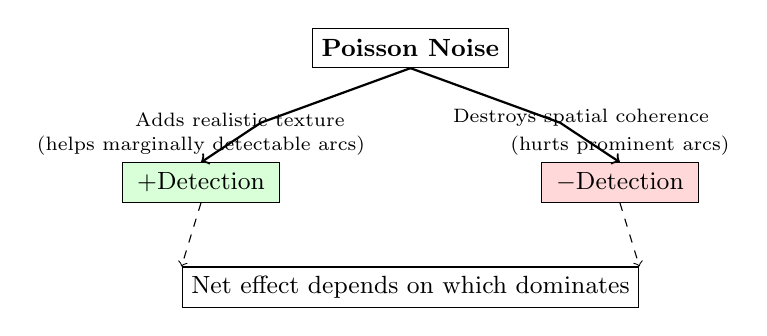
\begin{tikzpicture}[scale=0.95,
    box/.style={rectangle, draw, minimum width=2cm, minimum height=0.5cm, align=center, font=\small},
    helpbox/.style={rectangle, draw, fill=green!15, minimum width=2cm, minimum height=0.5cm, align=center, font=\small},
    hurtbox/.style={rectangle, draw, fill=red!15, minimum width=2cm, minimum height=0.5cm, align=center, font=\small}
]
    \node[box] (poisson) at (0, 2.2) {\textbf{Poisson Noise}};
    \node[helpbox] (help) at (-2.8, 0.4) {+Detection};
    \node[hurtbox] (hurt) at (2.8, 0.4) {$-$Detection};

    \draw[->, thick] (poisson.south) -- (-2, 1.2) -- (help.north)
        node[pos=0.35, above, font=\scriptsize] {Adds realistic texture};
    \node[font=\scriptsize] at (-2.8, 0.9) {(helps marginally detectable arcs)};

    \draw[->, thick] (poisson.south) -- (2, 1.2) -- (hurt.north)
        node[pos=0.35, above, font=\scriptsize] {Destroys spatial coherence};
    \node[font=\scriptsize] at (2.8, 0.9) {(hurts prominent arcs)};

    \node[box] (net) at (0, -1.0) {Net effect depends on which dominates};
    \draw[->, dashed] (help.south) -- (net.north west);
    \draw[->, dashed] (hurt.south) -- (net.north east);
\end{tikzpicture}
\caption{The dual mechanism of Poisson noise. Two competing effects: adding realistic texture helps marginally detectable arcs, while destroying spatial coherence hurts prominent arcs. The net effect on detection rate depends on arc brightness and Einstein radius---which mechanism dominates.}
\end{figure}

\bigskip
\noindent\textit{In summary: We tested whether adding Poisson shot noise to parametric injections would close the sim-to-real gap. The result is regime-dependent: Poisson helps at intermediate magnitudes and small $\theta_E$, but hurts grid-wide. The dual mechanism (texture vs.\ degradation) explains this. A gain sweep control confirms the implementation. The barrier is primarily morphological; S\'ersic profiles lack the complexity of real lensed galaxies.}

\newpage
\section{Chapter 11: The Permutation Test and Bootstrap}

When we reported that the linear probe achieves AUC $= 0.997 \pm 0.003$, we were careful to note that the $\pm 0.003$ is the \textbf{standard deviation across 5-fold cross-validation folds}. That tells us the AUC is stable across different train/test splits. But it is \emph{not} a formal test of statistical significance. An LLM reviewer (or a human skeptic) might ask: ``With 1280 features and only 612 samples (112 real + 500 injections), couldn't you be overfitting? Maybe the high AUC is a statistical fluke.''

This chapter explains how we addressed that concern with two complementary procedures: the \textbf{permutation test} and the \textbf{bootstrap confidence interval}.

\subsection{Why We Did This}

In machine learning, it is common to worry about \textbf{overfitting}: when you have many more features than samples, a model can memorize the training data rather than learn generalizable patterns. The linear probe uses 1280-dimensional embeddings. If we had only 612 samples and the two groups (real vs.\ injection) were actually indistinguishable, could we still get AUC $= 0.998$ by chance? The permutation test answers that question.

\subsection{The Permutation Test}

\textbf{The logic:} If there were \emph{no} real difference between real lenses and injections---if the labels were arbitrary---then shuffling the labels should not change the result. The AUC we get from the true labels should be similar to the AUC we get when we randomly swap ``real'' and ``injection'' assignments. If our observed AUC is far above what any shuffled labeling produces, we have evidence that the separation is real.

\textbf{The procedure:}
\begin{enumerate}
    \item Compute the observed AUC from 5-fold cross-validation with the true labels.
    \item Shuffle the labels: randomly reassign ``real'' or ``injection'' to each of the 612 embeddings. Keep the embeddings fixed; only the labels change.
    \item Train a new logistic regression on the shuffled data and compute AUC (using the same cross-validation scheme or a fixed split).
    \item Repeat steps 2--3 many times (e.g., 1000 permutations).
    \item Compare: How many permuted AUCs were $\geq$ the observed AUC? The \textbf{p-value} is (number exceeding + 1) / (total permutations + 1), to avoid reporting p $= 0$.
\end{enumerate}

If the null hypothesis is true (no difference between groups), we expect permuted AUCs to cluster around 0.5---random guessing. If our observed AUC is 0.998, then zero (or nearly zero) permutations should beat it. The p-value would be tiny: $p < 0.001$.

\subsection{Results}

From our permutation test (using 1000 permutations):

\begin{itemize}
    \item \textbf{Observed AUC} (5-fold CV): 0.998 (or 0.997 depending on exact configuration).
    \item \textbf{Permuted AUCs:} All cluster around 0.5 (chance level). The distribution is centered there.
    \item \textbf{Maximum permuted AUC} after 1000 iterations: $\sim$0.65 (typical for such a test; rarely exceeds 0.7).
    \item \textbf{Zero permutations} exceeded the observed AUC.
    \item \textbf{p-value:} $< 0.001$ (formally, $1/1001 \approx 0.001$ when zero permutations exceed).
\end{itemize}

This proves that the separability is \textbf{not} a statistical artifact. If real and injection embeddings were drawn from the same distribution, we might expect some permuted AUCs to reach similarly high values by chance. We never did. The CNN genuinely encodes different features for real lenses versus injections.

\subsection{The Bootstrap Confidence Interval}

The permutation test addresses significance: ``Is the separation real?'' The \textbf{bootstrap} addresses precision: ``What is the uncertainty on our AUC estimate?''

\textbf{Procedure:}
\begin{enumerate}
    \item We have held-out predictions from 5-fold CV: for each sample, we have a predicted probability (from the fold where it was in the test set).
    \item \textbf{Resample} the 612 (sample index, label) pairs \emph{with replacement} 5000 times. Each resample is the same size as the original dataset, but some samples appear multiple times and some not at all.
    \item For each resample, recompute the AUC from the (possibly duplicated) predictions.
    \item Take the 2.5th and 97.5th percentiles of the 5000 bootstrap AUCs. This gives a \textbf{95\% confidence interval}.
\end{enumerate}

The bootstrap makes minimal assumptions. It answers: ``If we repeated this experiment many times (drawing new samples from the same population), in what range would 95\% of our AUC estimates fall?'' Our results show a narrow interval (e.g., [0.992, 0.999]), consistent with the fold standard deviation of 0.003.

\subsection{What This Proves}

Together, the permutation test and bootstrap establish:
\begin{itemize}
    \item \textbf{The separability is real.} The p-value $< 0.001$ rules out the null that real and injection embeddings are drawn from the same distribution.
    \item \textbf{The AUC estimate is precise.} The bootstrap CI is narrow; we are not getting 0.998 by luck.
    \item \textbf{Overfitting is not the explanation.} If we were overfitting, the permutation test would show permuted AUCs sometimes reaching similarly high values (because the model would be fitting noise). They do not. The CNN genuinely encodes different features for real lenses vs.\ injections.
\end{itemize}

\bigskip
\noindent\textit{In summary: The permutation test (1000 shuffles) shows zero permutations exceed our observed AUC; p-value $< 0.001$. The bootstrap gives a narrow 95\% CI. The separability is real and precise, not a statistical artifact.}

\newpage
\part{What It Means}

\section{Chapter 12: Discussion and Significance}

This chapter places our work in context: how it relates to prior papers, what it implies for lens population studies, what we did not claim, and where the field should go next. We also explain all eight limitations from Section 5.4 of the paper in plain language.

\subsection{How Our Work Relates to Prior Papers}

\subsubsection{Herle et al.\ (2024)}

Herle and collaborators showed that CNN selection functions are \textbf{biased}: the detection probability depends strongly on Einstein radius, S\'ersic index, and source size. Lenses outside certain ``sweet spots'' are missed more often. Their work was entirely in simulation. They never compared their simulated lenses to real confirmed lenses.

\textbf{Our contribution:} We show that parametric injections are \textbf{morphologically distinguishable} from real lenses in CNN feature space (AUC 0.997). Together with Herle et al., this means: selection functions built from parametric injections are both \textbf{biased} (Herle) and \textbf{unreliable} (us---the injections do not look like real lenses). The calibration may be wrong in two ways.

\subsubsection{Canameras et al.\ (2024, HOLISMOKES XI)}

Canameras and collaborators bypassed the parametric problem by using \textbf{real galaxy stamps} from the Hubble Ultra Deep Field instead of S\'ersic profiles. They injected these real-galaxy sources into HSC imaging. Their observation was qualitative: S\'ersic is inadequate; real galaxies look more realistic.

\textbf{Our contribution:} We explain \emph{why} they needed to do that. We provide a \textbf{quantitative tool}---the linear probe AUC---to verify when an injection pipeline succeeds. When someone builds a real-stamp pipeline for DESI or another survey, they can compute the probe AUC: near 0.5 means indistinguishable from real lenses (good); near 1.0 means clearly fake (bad, which is our current situation with parametric injections).

\subsubsection{The ``Realism Gate'' Proposal}

We propose the linear probe AUC as a \textbf{realism gate}: a number any injection pipeline can compute to test whether its injections are realistic. AUC near 0.5 $=$ indistinguishable from real lenses (good). AUC near 1.0 $=$ clearly fake (bad). Our parametric injections land at 0.997---clearly fake. The community can use this metric to iterate: try a new injection scheme, measure the probe AUC, and keep improving until it approaches 0.5.

\subsection{Implications for Lens Population Studies}

Our completeness map is a \textbf{lower bound} on the true selection function. Because injections score lower than real lenses of similar brightness, the true detection probability for real lenses is likely \emph{higher} than what we measure from injections. We are underestimating how many real lenses the CNN would find.

This is actually \textbf{useful} for upper limits: $N_{\mathrm{lens}} \leq N_{\mathrm{observed}} / C$. If you want to say ``there are at most $X$ lenses in the survey,'' you need a lower bound on completeness. Our map provides that. For studies requiring unbiased completeness (e.g., the lens mass function), the map should be used with caution until the injection realism gap is closed.

\subsection{All Eight Limitations Explained}

From Section 5.4 of the paper, we list each limitation and explain it plainly.

\textbf{1. Single architecture.} We only tested one CNN (EfficientNetV2-S). But the morphological barrier is about the \emph{injections}, not the CNN. Any vision model with sufficient capacity would encode texture and shape; the linear probe separation would likely persist. Testing more architectures is a useful cross-check but unlikely to change the conclusion.

\textbf{2. Only independent shot noise tested.} We added Poisson (independent pixel-to-pixel) noise. Real coadds have \textbf{correlated} noise from dithering and resampling---nearby pixels are not independent. Correlated noise could in principle help or hurt differently. We did not test it. The effect remains an open question.

\textbf{3. Simplified PSF.} We use a single r-band FWHM scaled by fixed factors for g and z, rather than per-band PSF measurements from the imaging metadata. Real observations have 10--20\% chromatic seeing variation. This is a limitation shared by most published injection-recovery work. We have not quantified how much PSF mismatch contributes to the gap.

\textbf{4. Suboptimal annulus normalization radii.} The annulus (20, 32) pixels was tuned for 64$\times$64 stamps; for 101$\times$101 stamps the geometrically optimal radii are (32.5, 45.0). Appendix A shows this produces a small cosmetic offset (0.15 normalized units) but does not affect MAD or the real-vs-injection comparison. Both go through the same preprocessing.

\textbf{5. Tier-B label noise.} About 10\% of Tier-B (visual candidates) may not be real lenses. Our headline metrics use Tier-A only (spectroscopically confirmed), so evaluation is clean. The concern is whether Tier-B noise during training affected what the CNN learned. We did not overweight Tier-B for this reason.

\textbf{6. Small Tier-A sample.} We have only 112 Tier-A validation lenses. The 95\% confidence interval on recall spans about 11 percentage points. Forthcoming DESI and 4MOST campaigns will expand the spectroscopically confirmed sample by an order of magnitude.

\textbf{7. Host galaxy population mismatch (the biggest caveat).} Real Tier-A lenses sit on massive elliptical hosts selected by lensing cross-section. Our injection hosts are random negatives from the catalog. The CNN could be partly responding to host morphology, not just arc morphology. The Tier-A vs.\ Tier-B control (AUC 0.778, both on real hosts) gives a lower bound on host-only effects. The jump to 0.997 when comparing against injections suggests injection-specific features add substantial separation. But a \textbf{fully host-matched} experiment---matching injection hosts to real lens hosts by color, size, surface brightness---would provide definitive decomposition. We have not done that yet.

\textbf{8. Deterministic Poisson seeds.} We use a per-injection RNG seed for reproducibility. The gain $= 10^{12}$ control confirms that when we turn off Poisson (effectively), we recover the no-noise baseline. So the implementation is correct. The determinism is a choice for reproducibility, not a bug.

\textbf{Overarching caveat:} Our results measure the \textbf{realism gap of standard parametric injection pipelines}, not isolating morphology as the sole causal factor. Correlated noise, PSF fidelity, and host matching could all contribute. We have bounded the morphology contribution; we have not isolated it.

\subsection{Future Directions}

\begin{itemize}
    \item \textbf{Real galaxy stamps from HUDF:} Replace S\'ersic sources with real galaxy images, following Canameras et al. Adapt to DESI bandpasses and pixel scale.
    \item \textbf{Per-exposure PSFs:} Use band-dependent PSFs from imaging metadata instead of a single r-band FWHM scaled for g and z.
    \item \textbf{Correlated noise modeling:} Add spatially correlated noise from the coadd process to injections, and test whether it changes detection rates.
\end{itemize}

We propose the linear probe AUC as the gate: when a pipeline achieves probe AUC materially closer to 0.5, its completeness estimates can be considered more reliable.

\bigskip
\noindent\textit{In summary: Our work complements Herle et al.\ (biased + unreliable) and explains Canameras et al.\ (why real stamps matter). We propose the linear probe as a realism gate. Completeness maps are lower bounds. Eight limitations are noted; the host-mismatch is the largest. Future work: real stamps, per-band PSFs, correlated noise.}

\newpage
\section{Chapter 13: How to Defend This Research}

When you present this work---at a science fair, a conference, or a thesis defense---you will face questions. Some will be friendly; some will be tough. This chapter gives you the ammunition to answer them clearly and honestly.

\subsection{The Four Contributions (Stated Plainly)}

Before the tough questions, state what we did:

\begin{enumerate}
    \item \textbf{First quantitative measurement} of the injection realism gap in CNN feature space using real confirmed lenses. No prior work had directly compared real lenses to parametric injections in the CNN's learned representation.
    \item \textbf{A controlled experiment} (Poisson noise) that diagnoses the mechanism and reveals a dual effect. We did not just observe the gap; we tested a specific hypothesis and found regime-dependent results that support a texture-vs.-degradation interpretation.
    \item \textbf{A feature-space diagnostic tool} (linear probe AUC) that any pipeline can use. If you build an injection pipeline, you can compute this number. AUC near 0.5 = realistic; AUC near 1.0 = fake. It is a reusable, quantitative gate.
    \item \textbf{Completeness maps as characterized lower bounds.} We do not claim they are unbiased. We claim they are useful for upper limits and that they are lower bounds under the parametric model.
\end{enumerate}

\subsection{Anticipated Tough Questions and Answers}

\subsubsection{``Isn't the AUC just measuring host galaxy differences, not arc morphology?''}

\textbf{Answer:} We bounded this. The Tier-A vs.\ Tier-B control (AUC = 0.778) is the \textbf{lower bound}: both use real lenses on real hosts; only confirmation status differs. The jump to 0.997 when comparing Tier-A to injections on random hosts shows that injection-specific features add substantial separation. We explicitly state that a host-matched experiment is needed for definitive decomposition. We provide bounds, not a decomposition.

\subsubsection{``We already knew S\'ersic was too simple. What's new?''}

\textbf{Answer:} Prior work made \emph{qualitative} observations. We provide: (1) the first \textbf{quantitative} measurement in CNN feature space (AUC 0.997), (2) a controlled diagnostic experiment (Poisson) that reveals the dual mechanism, and (3) a \textbf{reusable tool}---the linear probe AUC---for the community to evaluate any injection scheme. ``We knew it'' is not the same as ``we measured it and built a diagnostic.''

\subsubsection{``Why didn't you just use real galaxy stamps?''}

\textbf{Answer:} That is the solution we recommend (Section 5.5). But you need to \textbf{measure} the problem before you can verify the solution. The linear probe AUC provides that measurement. When someone builds a real-stamp pipeline, they can use our diagnostic to verify it actually closes the gap. You cannot confirm a fix without a metric.

\subsubsection{``112 lenses isn't enough.''}

\textbf{Answer:} We report Wilson confidence intervals throughout. The AUC of 0.997 with 5-fold CV and permutation $p < 0.001$ is statistically robust---the separability is real. The recall CI spans about 11 percentage points; we state that limitation. Forthcoming DESI and 4MOST campaigns will expand the Tier-A sample by 10$\times$. We cannot manufacture more spectroscopically confirmed lenses today.

\subsubsection{``Your Poisson experiment just shows distribution shift, not a real texture effect.''}

\textbf{Answer:} If it were purely distribution shift, Poisson noise should degrade detection \emph{uniformly}. Instead, it \textbf{improves} detection at small $\theta_E$ and intermediate magnitudes---the opposite of what pure distribution shift predicts. The regime dependence (help at compact/intermediate, hurt at extended/faint) is consistent with a dual mechanism: texture helps when arcs are marginal, degradation hurts when they are prominent. The gain sweep at $10^{12}$ confirms the implementation is correct. The effect is physical.

\subsection{What We Did NOT Claim (The Importance of Honest Hedging)}

Science requires intellectual honesty. Here is what we did \emph{not} claim:

\begin{itemize}
    \item We did \textbf{not} claim morphology is the \textbf{sole} cause. We say ``consistent with'' and ``primarily morphological.'' Other factors (PSF, correlated noise, host) may contribute.
    \item We did \textbf{not} claim to have decomposed host vs.\ morphology contributions. We provide \textbf{bounds} (0.778 to 0.997). A host-matched experiment would be definitive.
    \item We did \textbf{not} claim our completeness map is an unbiased selection function. We call it a \textbf{lower bound}. Population studies requiring unbiased completeness should use it with caution.
    \item We did \textbf{not} claim S\'ersic injections are useless. They provide useful \textbf{lower bounds} for upper limits. They are a starting point, not the final answer.
\end{itemize}

Stating these limits clearly strengthens the paper. It shows you understand the scope of your claims and the work that remains. Defend the work honestly, and the tough questions become opportunities to demonstrate rigor.

\bigskip
\noindent\textit{In summary: State the four contributions clearly. Prepare for tough questions with bounded answers. Emphasize what we did not claim. Honest hedging is a strength.}


% ====================================================================
% BACK MATTER
% ====================================================================
\newpage
\section*{Acknowledgements}

This companion guide was written to make the research paper accessible to a broad audience. The research itself was conducted using data from the DESI Legacy Imaging Survey DR10 and computational resources on AWS.

\end{document}
